\begin{abox}
	Net-2019 
\end{abox}
\begin{enumerate}
	\item In a bacterial cell, a protein is synthesized at random location in the cytoplasm. The protein has to reach one pole of the cell for its appropriate function. The protein reaches the pole by
	 \begin{tasks}(2)
		\task[\textbf{a.}]Chemical attraction
		\task[\textbf{b.}]Random movement
		\task[\textbf{c.}]Enzymatic action
		\task[\textbf{d.}] Attraction between opposite charges
	\end{tasks}
\begin{answer}
	So the correct answer is \textbf{Option (b)}
\end{answer}
	\item A precious stone breaks into four pieces having weights in the proportion $1: 2: 3: 4$. The value of such a stone is proportional to the square of its weight. What is the percent loss in the value incurred due to breaking?
	 \begin{tasks}(4)
		\task[\textbf{a.}]0
		\task[\textbf{b.}]30
		\task[\textbf{c.}]70
		\task[\textbf{d.}] 90
	\end{tasks}
\begin{answer}
	\begin{align*}
	\text{ Weight of four pieces are }&k, 2 k, 3 k, 4 k\\
	\text{Total weight of all four pieces }&=10 k\\
\text{	The value of original piece }&=100 \alpha k^{2},\text{ where} \alpha\text{ is proportionality constant}\\
\text{	Total value of pieces after breaking }&=\alpha k^{2}+4 \alpha k^{2}+9 \alpha k^{2}+16 \alpha k^{2}=30 \alpha k^{2}\\
	\text{Percentage loss in value }&=\frac{70 \alpha k^{2}}{100 \alpha k^{2}} \times 100=70 \%
	\end{align*}
	So the correct answer is \textbf{Option (c)}
\end{answer}
	\item Two runners starting together run on a circular path taking 6 and 8 minutes, respectively, to complete one round. How many minutes later do they meet again for the first time on the start line, assuming constant speeds
	 \begin{tasks}(4)
		\task[\textbf{a.}]8
		\task[\textbf{b.}]24
		\task[\textbf{c.}]32
		\task[\textbf{d.}] 60
	\end{tasks}
\begin{answer}
	Solution: The required time is the LCM of $6 \mathrm{~min}$ and $8 \mathrm{~min}$\\
	Therefore time to meet again at the start time $=24 \mathrm{~min}$\\
		So the correct answer is \textbf{Option (b)}
\end{answer}
	\item 	 The distribution of grades secured by students in a class is given in the table below.\\\\
	\renewcommand*{\arraystretch}{1.2}
	\begin{tabular}{|c|c|}
		\hline Grade & Fraction of the Population \\
		\hline A & $0.1$ \\
		\hline B & $0.4$ \\
		\hline C & $0.3$ \\
		\hline D & $0.2$ \\
		\hline
	\end{tabular}\\\\
	What is the least possible population of the class?
	 \begin{tasks}(4)
		\task[\textbf{a.}]2
		\task[\textbf{b.}]4
		\task[\textbf{c.}]8
		\task[\textbf{d.}] 10
	\end{tasks}
\begin{answer}
 The number of students obtaining a grade must be a whole number.\\
	Options (a), (b) and (c) gives the number of students obtaining a grade as a fractional number. Hence option (d) is the correct answer.\\
	So the correct answer is \textbf{Option (d)}
\end{answer}
\item  The nine numbers $x_{1}, x_{2}, x_{3} \ldots x_{9}$, are in ascending order. Their average $m$ is strictly greater than all the first eight numbers. Which of the following is true?
	 \begin{tasks}(1)
		\task[\textbf{a.}]Average $\left(x_{1}, x_{2} \ldots x_{9}, m\right)>m$ and Average $\left(x_{2}, x_{3}, \ldots x_{9}\right)>m$
		\task[\textbf{b.}] Average $\left(x_{1}, x_{2} \ldots x_{9}, m\right)<m$ and Average $\left(x_{2}, x_{3}, \ldots x_{9}\right)<m$
		\task[\textbf{c.}] Average $\left(x_{1}, x_{2} \ldots x_{9}, m\right)=m$ and Average $\left(x_{2}, x_{3}, \ldots x_{9}\right)>m$
		\task[\textbf{d.}] Average $\left(x_{1}, x_{2} \ldots x_{9}, m\right)<m$ and Average $\left(x_{2}, x_{3}, \ldots x_{9}\right)=m$
	\end{tasks}
\begin{answer}
	\begin{align}
\text{ From the question}\notag\\
	x_{1}+x_{2}+\ldots x_{9}&=9 m \label{N-1} \\
	\text { and } x_{1}+x_{2}+\ldots x_{9}+m&=10 \alpha \label{N-2} \\
\text{	where $\alpha$ is the assumed }&\text{average of first 9 numbers and number $m$}\notag\\
\text{	From equation (\ref{N-1}) and (\ref{N-2});} &\text{$9 m+m=10 \alpha \Rightarrow \alpha=m$}\notag\\
\text{	Let $\beta$ be the average of }&x_{2}, x_{3} \ldots x_{9}. \text{ Then}\notag\\
\alpha_{2}+x_{3}+\ldots x_{9}&=8 \beta \label{N-3} \\
\text{From equations (\ref{N-1}) and (\ref{N-3})}\notag\\
8 \beta=9 m-x_{1}&=8 m+\left(m-x_{1}\right)\notag\\
\text{or }\beta=m&+\frac{m-x_{1}}{8}\notag\\
\text{Since $m>x_{1} $\quad}&\text{ therefore }\beta>m\notag
	\end{align}
	So the correct answer is \textbf{Option (c)}
\end{answer}
\item  Which among the following diagrams represents women, mothers, human beings?
	 \begin{tasks}(2)
		\task[\textbf{a.}]
		\begin{figure}[H]
			\centering
			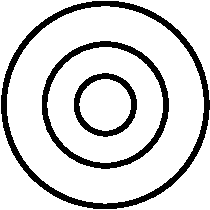
\includegraphics[height=2cm,width=2cm]{Net-19-1}
		\end{figure}
		\task[\textbf{b.}]
		\begin{figure}[H]
			\centering
			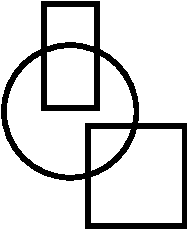
\includegraphics[height=2.4cm,width=2cm]{Net-19-2}
		\end{figure}
		\task[\textbf{c.}]
		\begin{figure}[H]
			\centering
			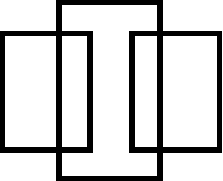
\includegraphics[height=2cm,width=2cm]{Net-19-3}
		\end{figure}
		\task[\textbf{d.}] 
		\begin{figure}[H]
			\centering
			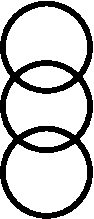
\includegraphics[height=2.3cm,width=1cm]{Net-19-4}
		\end{figure}
	\end{tasks}
\begin{answer}
All mothers are women and all wemen are human being\\
	So the correct answer is \textbf{Option (a)}
\end{answer}
\item  A boy and a girl make the following statements, of which at most one is correct:
The one in a white shirt says: "I am a girl" (statement - I)
The one in a blue shirt says: "I am a boy" (statement - II)
Which of the following is the correct inference?
	 \begin{tasks}(1)
		\task[\textbf{a.}]Statement - I is correct but statement - II is incorrect
		\task[\textbf{b.}]Statement - II is correct but statement - I is incorrect
		\task[\textbf{c.}]Both statement I and II are incorrect
		\task[\textbf{d.}] The correctness of the statements I and II cannot be ascertained	
	\end{tasks}
\begin{answer}
	From the wording of question, at least one statement is incorrect. If (I) is incorrect then (II) must be incorrect and vice-versa. If we take both statements to be incorrect this no contradiction.\\
	So the correct answer is \textbf{Option (c)}
\end{answer}
\item  How many quadrilaterals does the following figure have?	
\begin{figure}[H]
	\centering
	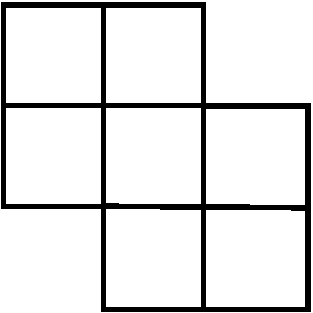
\includegraphics[height=2cm,width=2cm]{Net-19-5}
\end{figure}
 \begin{tasks}(4)
	\task[\textbf{a.}]17
	\task[\textbf{b.}]18
	\task[\textbf{c.}]19
	\task[\textbf{d.}] 20
\end{tasks}
\begin{answer}$\left. \right. $
	\begin{figure}[H]
		\centering
		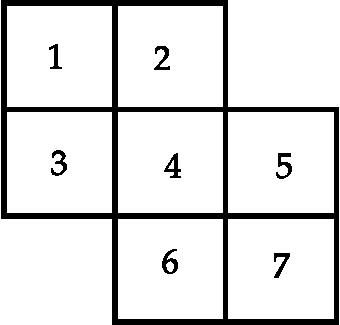
\includegraphics[height=2cm,width=2.2cm]{Net-19-33}
	\end{figure}
	\begin{align*}
	&\text{ The quadrilaterals formed are}\\
	&1,1+2,1+3 \\
	&1+2+3+4,2,2+4 \\
	&2+4+6,3+4,3+4+5,4+5 \\
	&4+6,4+5+6+7,5+7,6+7 \\
	&3,4,5,6,7
	\text{This total number of quadrilaterals formed are $19 .$}
	\end{align*}
		So the correct answer is \textbf{Option (c)}
\end{answer}
\item  12 balls, 3 each of the colours red, green, blue and yellow are put in a box and mixed. If 3 balls are picked at random, without replacement, the probability that all 3 balls are of the same colour is
 \begin{tasks}(4)
	\task[\textbf{a.}]$\frac{1}{4}$
	\task[\textbf{b.}] $\frac{1}{12}$
	\task[\textbf{c.}]$\frac{1}{36}$
	\task[\textbf{d.}]$\frac{1}{55}$ 
\end{tasks}
\begin{answer}
	\begin{align*}
	\text { The number of ways of drawing } 3 \text { balls is }{ }^{12} C_{3}=\frac{12 !}{3 ! 9 !}&=220\\
	\text{The number of ways of obtaining 3 balls are of the same colour} =4\\
\text{	Hence the probability that the 3 balls are of the same colour} =\frac{4}{220}&=\frac{1}{55}
	\end{align*}
		So the correct answer is \textbf{Option (d)}
\end{answer}
\item  Some aliens observe that roosters call before sunrise every day. Having no other information about roosters and sunrises, which of the following inferences would NOT be valid?
 \begin{tasks}(1)
	\task[\textbf{a.}]Rooster-call and sunrise may be independent cyclic events with the same periodicity
	\task[\textbf{b.}]Both may be triggered by a common cause
	\task[\textbf{c.}]Rooster-call may be causing the sunrise
	\task[\textbf{d.}]Sunrise cannot be the cause of rooster call as the rooster-call precedes sunrise 
\end{tasks}
\begin{answer}
	 In common life we assume that cause proceeds "effect" \\
	So the correct answer is \textbf{Option (d)}
\end{answer}
\item  Twenty-one litres of water in a tank is to be divided into three equal parts using only 5,8 and 12 litre capacity cans. The minimum number of transfers needed to achieve this is
 \begin{tasks}(4)
	\task[\textbf{a.}]3
	\task[\textbf{b.}]4
	\task[\textbf{c.}]5
	\task[\textbf{d.}] 7
\end{tasks}
\begin{answer}
	\begin{align*}
	21 L \rightarrow 7+7+7 ; \text { Cans Capacity }& 5,8,12\\
	\text { Minimum number of transfer }&=7
	\end{align*}
		So the correct answer is \textbf{Option (d)}
\end{answer}
\item  Of four agents Alpha, Beta, Gamma and Delta, three have to be sent together on a mission. If Alpha and Beta cannot go together, Beta and Gamma cannot go together and Gamma and Delta cannot go together, then which of the following holds?
 \begin{tasks}(1)
	\task[\textbf{a.}]Any three agents can be sent.
	\task[\textbf{b.}]Alpha, Delta and any one out of Beta and Gamma can be sent
	\task[\textbf{c.}] Beta, Gamma and any one out of Alpha and Delta can be sent
	\task[\textbf{d.}] The mission is impossible.
\end{tasks}
\begin{answer}
	According to the question it is impossible to form a team of 3 members as the conditions of the problem does not allow it.\\
So the correct answer is \textbf{Option (d)}
\end{answer}
\item  An open rectangular box is made by excluding the four identical corners of a piece of paper as shown in the diagram and folding it along the dotted lines
\begin{figure}[H]
	\centering
	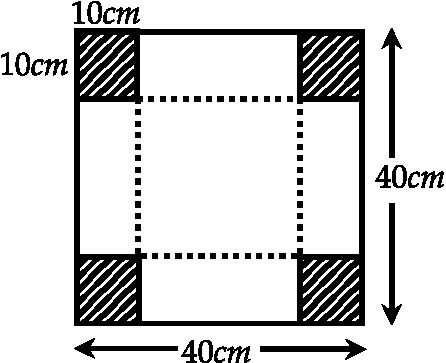
\includegraphics[height=3.1cm,width=4cm]{Net-19-6}
\end{figure}
The capacity of the box $\left(\mathrm{in} \mathrm{cm}^{3}\right)$ is
 \begin{tasks}(4)
	\task[\textbf{a.}] 8000
	\task[\textbf{b.}]1000
	\task[\textbf{c.}]4000
	\task[\textbf{d.}] 6000
\end{tasks}
\begin{answer}
	\begin{align*}
	\text { The length and width of the box are } &20 \mathrm{~cm} \text { and } 20 \mathrm{~cm} \text { while its heights is } 10 \mathrm{~cm} \text {. }\\
	\text { Hence capacity of the box is } 20 \times 20 \times 10&=4000 \mathrm{~cm}^{3}
	\end{align*}
	So the correct answer is \textbf{Option (c)}
\end{answer}
\item  Which of the following is the largest?
$
2^{50}, 3^{40}, 4^{30}, 5^{20}
$
 \begin{tasks}(4)
	\task[\textbf{a.}] $2^{50}$
	\task[\textbf{b.}]$3^{40}$
	\task[\textbf{c.}]$4^{30}$
	\task[\textbf{d.}]$5^{20}$ 
\end{tasks}
\begin{answer}
	\begin{align*}
	&2^{50}=\left(2^{5}\right)^{10}=32^{10} ; \qquad 3^{40}=\left(3^{4}\right)^{10}=81^{10}\\
	&4^{30}=\left(4^{3}\right)^{10}=64^{10} ; \qquad 5^{20}=\left(5^{2}\right)^{10}=25^{10}\\
	&\text { Hence } 3^{40} \text { is largest }
	\end{align*}
		So the correct answer is \textbf{Option (b)}
\end{answer}
\item  A monkey climbs a tree to eat fruits. The amount of energy gained from eating fruits and the energy spent in climbing on different branches have a relationship shown in the figure.
\begin{figure}[H]
	\centering
	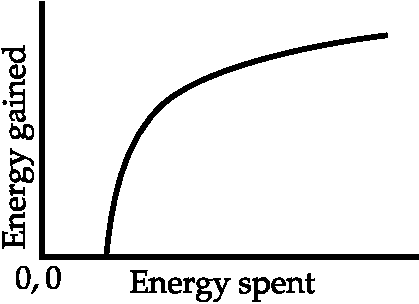
\includegraphics[height=2.1cm,width=3cm]{Net-19-7}
\end{figure}
The ratio of energy gained to energy spent will be the maximum
 \begin{tasks}(1)
	\task[\textbf{a.}] At a point where the slope of the curve is the maximum
	\task[\textbf{b.}] At a point where the slope of the curve is unity
	\task[\textbf{c.}]At a point on the curve where the tangent passes through the origin
	\task[\textbf{d.}] At the highest point on the curve
\end{tasks}
\begin{answer}
	So the correct answer is \textbf{Option (c)}
\end{answer}
\item  The length of a cylinder is measured 10 times yielding 10 distinct values. For this set of values, consider the following statements\\
A. Five of these values will lie above the mean and five below it\\
B. Five of these values will lie above median and five below it\\
C. At least one value will lie above the mean\\
D. At least one value will lie at the median\\
Which of the statements are necessarily correct?
 \begin{tasks}(4)
	\task[\textbf{a.}] $\mathrm{B}$ and $\mathrm{C}$
	\task[\textbf{b.}] $\mathrm{A}$ and $\mathrm{C}$
	\task[\textbf{c.}] B and D
	\task[\textbf{d.}]$\mathrm{A}, \mathrm{C}$ and $\mathrm{D}$ 
\end{tasks}
\begin{answer}
	It is not necessary that five of these values will lie above the mean and five below it. But since the observation  are distinct, we can arrange them in increasing or decreasing order; hence median will be the value between 5th 6th observation. It is the property of the mean that it must be less than the largest observtion if the observation are distinct.\\
	So the correct answer is \textbf{Option (a)}
\end{answer}
\item  In the given circle, $O$ is the centre, $\angle P A O=40^{\circ}, \angle P B Q=30^{\circ}$ and outer angle
$$
\angle A O B=220^{\circ} \text {. }
$$
Then $\angle A Q B$ is
\begin{figure}[H]
	\centering
	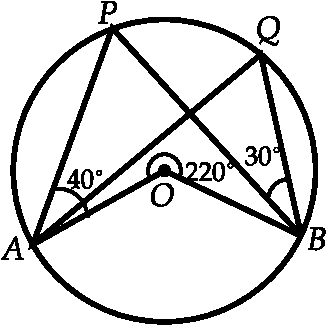
\includegraphics[height=3cm,width=3cm]{Net-19-8}
\end{figure}
 \begin{tasks}(4)
	\task[\textbf{a.}] $70^{\circ}$
	\task[\textbf{b.}] $80^{\circ}$
	\task[\textbf{c.}]$60^{\circ}$
	\task[\textbf{d.}] $110^{\circ}$
\end{tasks}
\begin{answer}
	\begin{align*}
	\text { The angle subtended by arc }& A M B \text { at the circle }\\
	&=360-220=140
	\intertext{From the fact that the angle subtended by an arc at the centre is double the angle subtended by it on the remaining part of the circle we obtain}
	\angle A Q B&=\frac{140^{\circ}}{2}=70^{\circ}
	\end{align*}
		So the correct answer is \textbf{Option (a)}
\end{answer}
\item  A canal system is shown in the figure
\begin{figure}[H]
	\centering
	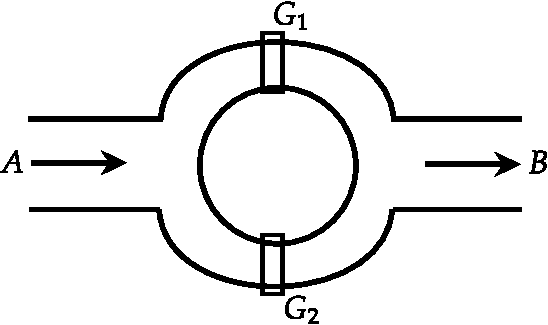
\includegraphics[height=2cm,width=3.5cm]{Net-19-9}
\end{figure}
Water flows from $A$ to $B$ through two channels. Gates $G_{1}$ and $G_{2}$, are operated independently to regulate the flow. Probability of $G_{1}$ to be open is $10 \%$ while that of $G_{2}$ is $20 \%$. The probability that water will flow from $A$ to $B$ is
 \begin{tasks}(4)
	\task[\textbf{a.}]$10 \%$
	\task[\textbf{b.}]$20 \%$
	\task[\textbf{c.}]$28 \%$
	\task[\textbf{d.}]$30 \%$
\end{tasks}
\begin{answer}
	\begin{align*}
&\text{Water will reach from A to B when}\\
&\text{	(I) $G_{1}$ is open and $G_{2}$ is closed}\\
&\text{	(II) $G_{1}$ is closed and $G_{2}$ is open}\\
&\text{	(III) Both $G_{1}$ and $G_{2}$ are open}\\
&\text{Hence probability that water flow from A to B is }\\
&0.1 \times 0.8+0.9 \times 0.2+0.1 \times 0.2=0.08+0.18+0.02=0.28=28 \%
	\end{align*}
		So the correct answer is \textbf{Option (c)}
\end{answer}
\item  A long ream of paper of thickness $t$ is rolled tightly. As the roll becomes larger, the length of the paper wrapped in one turn exceeds the length in the previous turn by
 \begin{tasks}(4)
	\task[\textbf{a.}]$t$
	\task[\textbf{b.}]$2 t$
	\task[\textbf{c.}]$\pi t$
	\task[\textbf{d.}] $2 \pi t$
\end{tasks}
\begin{answer}
 Let $r$ be the radius of the previous turn, then the radius of new turn will be $(r+t)$.
	Therefore the difference between the circumference of new turn and previous turn will $2 \pi(r+t)-2 \pi r=2 \pi t$\\
		So the correct answer is \textbf{Option (d)}
\end{answer}
 \item   Point $A$ on a wheel of radius $r$ touches the horizontal plane at point $P$. It rolls without slipping, till point $A$ is at the highest position in the first turn. What is the final distance $A P$ ?
 \begin{figure}[H]
 	\centering
 	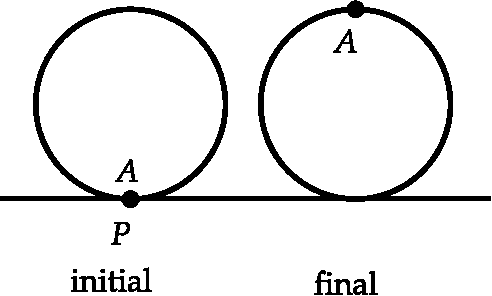
\includegraphics[height=2.4cm,width=4cm]{Net-19-10}
 \end{figure}
 \begin{tasks}(4)
	\task[\textbf{a.}]$2 r$
	\task[\textbf{b.}]$r \sqrt{\left(1+\pi^{2}\right)}$
	\task[\textbf{c.}] $r \sqrt{\left(4+\pi^{2}\right)}$
	\task[\textbf{d.}] $2 r \sqrt{\left(1+\pi^{2}\right)}$
\end{tasks}
\begin{answer}$\left. \right. $
	\begin{figure}[H]
		\centering
		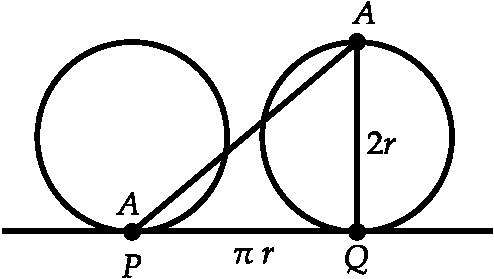
\includegraphics[height=2.5cm,width=4.5cm]{Net-19-34}
	\end{figure}
	\begin{align*}
	\intertext{ When point $P$ comes to the new position and becomes point $A$, the wheel makes half revolution and centre of the wheel moves by a distance $\pi r$}
\text{	Using Pythagoras }&\text{theorem in triangle $A P Q$ gives}\\
	A P&=\sqrt{(2 r)^{2}+(\pi r)^{2}}=r \sqrt{4+\pi^{2}}
	\end{align*}
		So the correct answer is \textbf{Option (c)}
\end{answer}
\item  An object is dropped on a cushion from a height $10 \mathrm{~m}$ above it. On being hit, the cushion is depressed by $0.1 \mathrm{~m}$. Assuming that the cushion provides a constant resistive force, the deceleration of the object after hitting the cushion, in terms of the acceleration due to gravity $g$ is
 \begin{tasks}(4)
	\task[\textbf{a.}]$10 g$
	\task[\textbf{b.}] $50 \mathrm{~g}$
	\task[\textbf{c.}] $100 \mathrm{~g}$
	\task[\textbf{d.}]  $g$
\end{tasks}
\begin{answer}$\left. \right. $
	\begin{figure}[H]
		\centering
		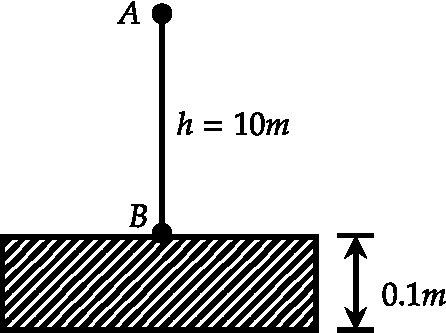
\includegraphics[height=3.1cm,width=4cm]{Net-19-35}
	\end{figure}
	\begin{align*}
	\text{From conservation}&\text{ at energy}\\
	m g h&=\frac{1}{2} m v^{2} \Rightarrow v=\sqrt{20 g}\\
	\text{The equation at }&\text{motion when partition the cushion}\\
	m v \frac{d v}{d x}&=m g-k \\
	\int_{\sqrt{20 g}}^{0} v d v&=\left.\int_{0.1}^{0}\left(g-\frac{k}{m}\right) d x \frac{v^{2}}{2}\right|_{\sqrt{20 g}} ^{0}=\left(g-\frac{k}{m}\right) \times 0.1 \\
	-\frac{20 g \times 0.1}{2}&=\left(g-\frac{k}{m}\right)=a-100 g=a
	\end{align*}
		So the correct answer is \textbf{Option (c)}
\end{answer}
\item  A turn-table is rotating with a constant angular velocity $\omega_{0}$. In the rotating frame fixed to the turntable, a particle moves radially outwards at a constant speed $v_{0}$. The acceleration of the particle in the $r \theta$ coordinates, as seen from an inertial frame, the origin of which is at the centre of the turntable, is
 \begin{tasks}(2)
	\task[\textbf{a.}]$-r \omega_{0}^{2} \hat{r}$
	\task[\textbf{b.}]$2 r \omega_{0}^{2} \hat{r}+v_{0} \omega_{0} \hat{\theta}$
	\task[\textbf{c.}]$r \omega_{0}^{2} \hat{r}+2 v_{0} \omega_{0} \hat{\theta}$
	\task[\textbf{d.}] $-r \omega_{0}^{2} \hat{r}+2 v_{0} \omega_{0} \hat{\theta}$
\end{tasks}
\begin{answer}
	\begin{align*}
	\text { The acceleration in Polar coordinate, } \vec{a}&=a_{r} \hat{r}+a_{\theta} \hat{\theta}=\left(\ddot{r}-r \dot{\theta}^{2}\right) \hat{r}+(r \ddot{\theta}+2 \dot{r} \dot{\theta}) \hat{\theta}\\
	\dot{r}=v_{0} \quad \ddot{r}=0 \text { and } \dot{\theta}&=\omega_{0} \quad \ddot{\theta}=0 \Rightarrow \vec{a}=\left(-r \omega_{0}^{2}\right) \hat{r}+\left(2 v_{0} \omega_{0}\right) \hat{\theta}
	\end{align*}
		So the correct answer is \textbf{Option (d)}
\end{answer}
\item  Assume that the earth revolves in a circular orbit around the sun. Suppose the gravitational constant $G$ varies slowly as a function of time. In particular, it decreases to half its initial value in the course of one million years. Then during this time the
(a) Radius of the earth's orbit will increase by a factor of two
(b) Total energy of the earth remains constant
(c) Orbital angular momentum of the earth will increase
(d) Radius of the earth's orbit remains the same.
\begin{answer}
	\begin{align*}
	G&=G(t) M \equiv \text { Mass of sun }, m=\text { mass of Earth }
	\intertext{The given Problem is central force problem so angular momentum of system is conserved. $J=C$}
\text{	Total}&\text{ Energy of system is}\\
	E&=\frac{1}{2} m \dot{r}^{2}+\frac{J^{2}}{2 m r^{2}}-\frac{G M m}{r}\\
\text{	Hence }G&=G(t)\text{ so }\frac{d E}{d t} \neq 0\text{ So total Energy }\text{is not conserve}\\
\text{	Condition }&\text{for circular motion}\\
	\frac{J^{2}}{m r^{3}}&=\frac{G M m}{r^{2}} \Rightarrow r \propto \frac{1}{G} \Rightarrow \frac{r_{2}}{r_{1}}=\frac{G_{1}}{G_{2}} \Rightarrow r_{2}=\frac{G_{1}}{G_{2}} r_{1} \Rightarrow r_{2}=\frac{G_{1} r_{1}}{\frac{G_{1}}{2}} \Rightarrow r_{2}=2 r_{1}
	\end{align*}
		So the correct answer is \textbf{Option (a)}
\end{answer}
\item  A particle of mass $m$ moves in One dimension in the potential $V(x)=k x^{4},(k>0)$. At time $t=0$ the particle starts from rest at $x=A$.
For bounded motion, the time period of its motion is
 \begin{tasks}(2)
	\task[\textbf{a.}]Proportional to $A^{-1 / 2}$
	\task[\textbf{b.}]Proportional to $A^{-1}$
	\task[\textbf{c.}] Independent of $A$
	\task[\textbf{d.}]  Not well-defined (the system is chaotic)
\end{tasks}
\begin{answer}
	\begin{align*}
	J&=\oint p d x \Rightarrow J=4 \int_{0}^{\left(\frac{E}{k}\right)^{1 / 4}} \sqrt{2 m\left(E-k x^{4}\right)} d x\\
	\frac{p^{2}}{2 m}+k x^{4}&=E \Rightarrow J \propto 4 \sqrt{2 m E}\left(\frac{E}{k}\right)^{1 / 4}\\
	p=0, x=A \Rightarrow E&=k A^{4}, \quad J \propto E^{3 / 4} \Rightarrow T=\frac{d J}{d E} \propto E^{-1 / 4} \quad T=k A^{-1}\\
	T&=k A^{-1} \quad T \propto \frac{1}{A}
	\end{align*}
		So the correct answer is \textbf{Option (b)}
\end{answer}
\item  The infinite square-well potential of a particle in a box of size a is modified as shown in the figure below (assume $\Delta<<a$ )
\begin{figure}[H]
	\centering
	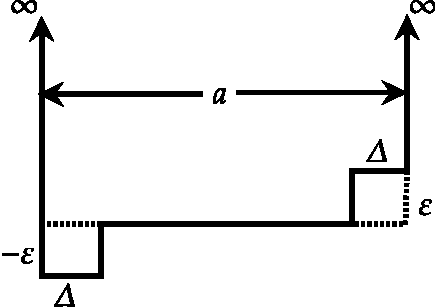
\includegraphics[height=2.7cm,width=3.5cm]{Net-19-11}
\end{figure}
The energy of the ground state, compared to the ground state energy before the perturbation was added
 \begin{tasks}(2)
	\task[\textbf{a.}]Increases by a team of order $\varepsilon$
	\task[\textbf{b.}] Decreases by a term of order $\varepsilon$
	\task[\textbf{c.}]Increases by a term of order $\varepsilon^{2}$
	\task[\textbf{d.}]  Decreases by a term of order $\varepsilon^{2}$
\end{tasks}
\begin{answer}
	\begin{align*}
	\text { The perturbation  }&\text{is anti-symmetric about centre at box}\\
\text{	So }E_{1}^{1}&=0\\
	E_{1}^{2}&=\sum_{m \neq 1} \frac{\left|\left\langle\varphi_{1}|w| \varphi_{m}\right\rangle\right|^{2}}{E_{1}^{0}-E_{m}^{0}}, E_{1}^{0}>E_{m}^{0} \text { so } E_{1}^{2}<0
	\end{align*}
		So the correct answer is \textbf{Option (d)}
\end{answer}
\item  A quantum particle of mass $m$ in one dimension, confined to a rigid box as shown in the figure, is in its ground state. An infinitesimally thin wall is very slowly raised to infinity at the centre of the box, in such a way that the system remains in its ground state at all times. Assuming that no energy is lost in raising the wall, the work done on the system when the wall is fully raised, eventually separating the original box into two compartments, is
\begin{figure}[H]
	\centering
	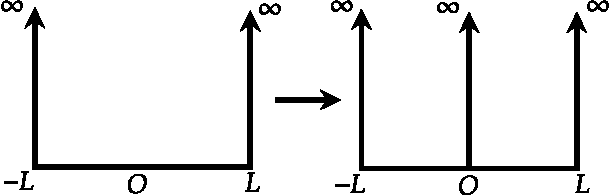
\includegraphics[height=2cm,width=5.8cm]{Net-19-12}
\end{figure}
 \begin{tasks}(4)
	\task[\textbf{a.}]$\frac{3 \pi^{2} \hbar^{2}}{8 m L^{2}}$
	\task[\textbf{b.}]$\frac{\pi^{2} \hbar^{2}}{8 m L^{2}}$
	\task[\textbf{c.}] $\frac{\pi^{2} \hbar^{2}}{2 m L^{2}}$
	\task[\textbf{d.}] 0
\end{tasks}
\begin{answer}
	\begin{align*}
	\text{Initial particle in ground state}\\
	E_{i}&=\frac{\pi^{2} \hbar^{2}}{2 m\left(2 L^{2}\right)}=\frac{\pi^{2} \hbar^{2}}{8 m L^{2}}
	\intertext{here the wall is introduced. Slowly the particle will in ground state at new wall with width }
	L E_{f}&=\frac{\pi^{2} \hbar^{2}}{2 m L^{2}}\\
	\Delta W&=E_{f}-E_{i}=\frac{\pi^{2} \hbar^{2}}{2 m L^{2}}-\frac{\pi^{2} \hbar^{2}}{8 m L^{2}}=\frac{3 \pi^{2} \hbar^{2}}{8 m L^{2}}
	\end{align*}
		So the correct answer is \textbf{Option (a)}
\end{answer}
\item  The wavefunction of a free particle of mass $m$, constrained to move in the interval $-L \leq x \leq L$, is $\psi(x)=A(L+x)(L-x)$, where $A$ is the normalization constant. The probability that the particle will be found to have the energy $\frac{\pi^{2} \hbar^{2}}{2 m L^{2}}$ is
 \begin{tasks}(4)
	\task[\textbf{a.}]0
	\task[\textbf{b.}]$\frac{1}{\sqrt{2}}$
	\task[\textbf{c.}]$\frac{1}{2 \sqrt{3}}$
	\task[\textbf{d.}] $\frac{1}{\pi}$ 
\end{tasks}
\begin{answer}
	\begin{align*}
	E_{n}&=\frac{x^{2} \pi^{2} \hbar^{2}}{8 m L^{2}} \Rightarrow E_{n}=\frac{n^{2} \pi^{2} \hbar^{2}}{8 m L^{2}}\\
	E_{1}&=\frac{\pi^{2} \hbar^{2}}{8 m L^{2}},\left|\phi_{1}\right\rangle=\sqrt{\frac{2}{2 L}} \cos \frac{\pi x}{2 L},-L \leq x \leq L \\
	E_{2}&=\frac{4 \pi^{2} \hbar^{2}}{8 m L^{2}}=\frac{\pi^{2} \hbar^{2}}{2 m L^{2}}=\sqrt{\frac{2}{2 L}} \sin \frac{2 \pi x}{2 L} \cdot-L \leq x \leq L \\
	P\left(E_{2}\right)&=\frac{\left|\left\langle\varphi_{2} \mid \psi\right\rangle\right|^{2}}{\langle\psi \mid \psi\rangle}\\
	&=\frac{\left|\int_{-L}^{L} \sqrt{\frac{2}{2 L}} \sin \frac{2 \pi x}{2 L} A(L+x)(L-x) d x\right|^{2}}{\int_{-L}^{L} A^{2}(L+x)^{2}(L-x)^{2} d x} \\
	&\int_{-L}^{L} \sin \frac{2 \pi x}{2 L}(L+x)(L-x) d x=0\\
	\text { where, }& \frac{2 \pi x}{2 L}(L+x)(L-x) \text { is odd }
	\end{align*}
		So the correct answer is \textbf{Option (a)}
\end{answer}
\item  A particle moving in a central potential is described by a wavefunction $\psi(r)=z f(r)$ where $r=(x, y, z)$ is the position vector of the particle and $f(r)$ is a function of $r=|r|$.
If $L$ is the total angular momentum of the particle, the value of $L^{2}$ must be
 \begin{tasks}(4)
	\task[\textbf{a.}]$2 \hbar^{2}$
	\task[\textbf{b.}]$\hbar^{2}$
	\task[\textbf{c.}]$4 \hbar^{2}$
	\task[\textbf{d.}]$\frac{3}{4} \hbar^{2}$ 
\end{tasks}
\begin{answer}
	\begin{align*}
	 \psi(r)&=z f(r)=r \cos \theta f(r)\\
	\cos \theta&=P_{1}(\cos \theta) \Rightarrow l=1 \\
	\psi(r, \theta, \varphi)&=P_{1}(\cos \theta) r f(r)\\
	\text{the measure at }&\text{$L^{2}$ have eigen value $l(l+1)$}\\ \hbar^{2} \quad\text{ put }l&=1 \quad 1(l+1) \hbar^{2}=2 \hbar^{2}
	\end{align*}
	So the correct answer is \textbf{Option (a)}
\end{answer}
\item  A particle of mass in and energy $E>0$. in one dimension is scattered by the potential below.
\begin{figure}[H]
	\centering
	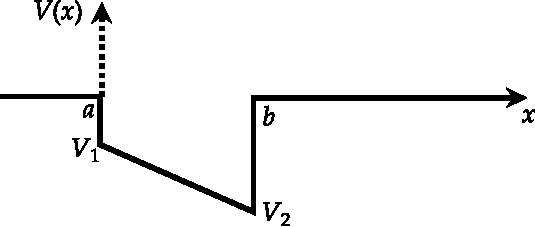
\includegraphics[height=2.3cm,width=5cm]{Net-19-13}
\end{figure}
If the particle was moving from $x=-\infty$ to $x=\infty$, which of the following graphs gives the best qualitative representation of the wavefunction of this particle?
 \begin{tasks}(2)
	\task[\textbf{a.}]
	\begin{figure}[H]
		\centering
		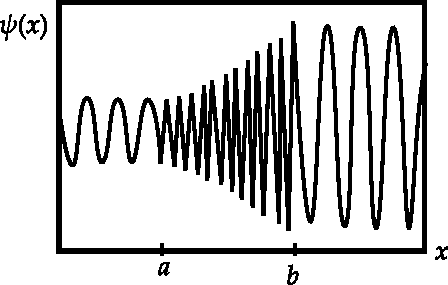
\includegraphics[height=3cm,width=5cm]{Net-19-14}
	\end{figure}
	\task[\textbf{b.}]
		\begin{figure}[H]
		\centering
		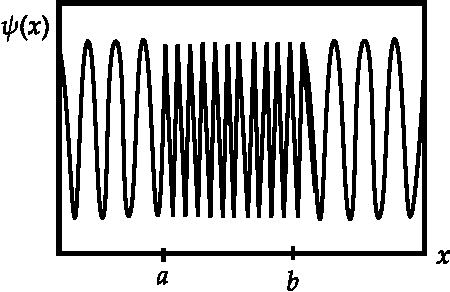
\includegraphics[height=3cm,width=5cm]{Net-19-15}
	\end{figure}
	\task[\textbf{c.}]
		\begin{figure}[H]
		\centering
		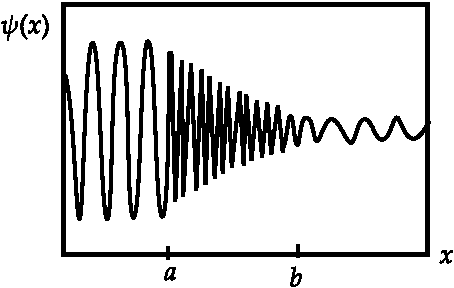
\includegraphics[height=3cm,width=5cm]{Net-19-16}
	\end{figure}
	\task[\textbf{d.}] 
		\begin{figure}[H]
		\centering
		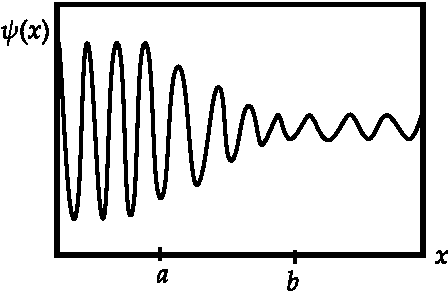
\includegraphics[height=3cm,width=5cm]{Net-19-17}
	\end{figure}
\end{tasks}
\begin{answer}
	So the correct answer is \textbf{Option (c)}
\end{answer}
\item  Consider a planar wire loop as an $n$-sided regular polygon, in which $R$ is the distance from the centre to a vertex. If a steady current $I$ flows through the wire, the magnitude of the magnetic field at the centre of the Loop is
 \begin{tasks}(4)
	\task[\textbf{a.}]$\frac{\mu_{0} I}{2 R} \sin \left(\frac{2 \pi}{n}\right)$
	\task[\textbf{b.}] $\frac{\mu_{0} n I}{4 \pi R} \sin \left(\frac{\pi}{n}\right)$
	\task[\textbf{c.}]$\frac{\mu_{0} n I}{2 \pi R} \tan \left(\frac{2 \pi}{n}\right)$
	\task[\textbf{d.}] $\frac{\mu_{0} n I}{2 \pi R} \tan \left(\frac{\pi}{n}\right)$
\end{tasks}
\begin{answer}$\left. \right. $
	\begin{figure}[H]
		\centering
		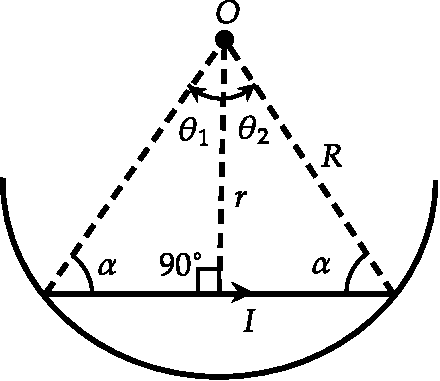
\includegraphics[height=3.5cm,width=4cm]{Net-19-36}
	\end{figure}
	\begin{align*}
	\text { Angle subtended by one side}&\text{ to the centre is } \frac{2 \pi}{n}\\
	\text { For segment (1), } B_{1}&=\frac{\mu_{0} I}{4 \pi r}\left[\sin \theta_{2}-\sin \theta_{1}\right]\\
	r&=R \sin \alpha, \theta_{1}=-(90-\alpha) \text { and } \theta_{2}=+(90-\alpha) \\
	\Rightarrow B_{1}&=\frac{\mu_{0} I}{4 \pi R \sin \alpha}[\cos \alpha+\cos \alpha]=\frac{\mu_{0} I}{2 \pi R} \cot \alpha\\
	\text { For } n \text {-sided polygon; } \alpha&=\frac{\pi}{2}-\frac{\pi}{n}\\
	\Rightarrow B_{1}&=\frac{\mu_{0} I}{2 \pi R} \tan \left(\frac{\pi}{n}\right)\\
\text{	Thus magnetic field due to }&\text{$n$-sided polygon is}\\
	B&=n B_{1}=\frac{n \mu_{0} I}{2 \pi R} \tan \left(\frac{\pi}{n}\right)
	\end{align*}
	So the correct answer is \textbf{Option (d)}
\end{answer}
\item  Two coherent plane electromagnetic waves of wavelength $0.5 \mu \mathrm{m}$ (both have the same amplitude and are linearly polarized along the $z$-direction) fall on the $y=0$ plane. Their wave vectors $k_{1}$ and $k_{1}$ are as shown in the figure
\begin{figure}[H]
	\centering
	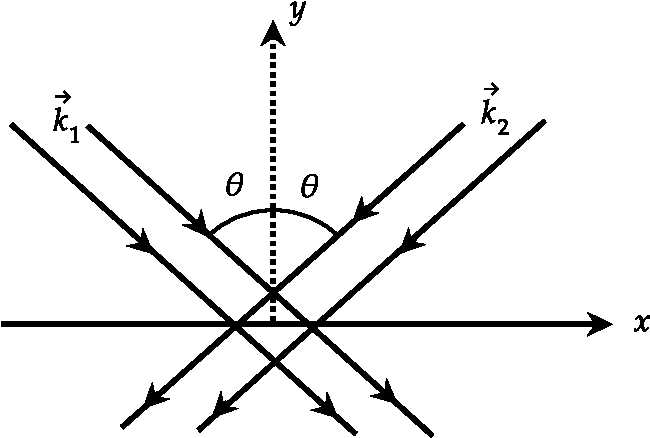
\includegraphics[height=3.3cm,width=5cm]{Net-19-18}
\end{figure}
If the angle $\theta$ is $30^{\circ}$, the fringe spacing of the interference pattern produced on the plane is
 \begin{tasks}(4)
	\task[\textbf{a.}]$1.0 \mu m$
	\task[\textbf{b.}]$0.29 \mu \mathrm{m}$
	\task[\textbf{c.}]$0.58 \mu \mathrm{m}$
	\task[\textbf{d.}]$0.5 \mu m$ 
\end{tasks}
\begin{answer}
	\begin{align*}
	\vec{E}_{1}&=\hat{z} A e^{i\left(\omega t-\vec{k}_{1} \cdot \vec{r}\right)} \text { and } \vec{E}_{2}=\hat{z} A e^{i\left(\omega t-\vec{k}_{2} \cdot \vec{r}\right)} \text { where }\left|\vec{k}_{1}\right|=\left|\vec{k}_{2}\right| \text {. }\\
	\vec{k}_{1}&=\left(k_{1} \sin \theta\right) \hat{x}-\left(k_{1} \cos \theta\right) \hat{y} \text { and } \vec{k}_{2}=-\left(k_{1} \sin \theta\right) \hat{x}-\left(k_{1} \cos \theta\right) \hat{y}\\
	\vec{k}_{1} \cdot \vec{r}&=\left(k_{1} \sin \theta\right) x-\left(k_{1} \cos \theta\right) y \text { and } \vec{k}_{2} \cdot \vec{r}=-\left(k_{1} \sin \theta\right) x-\left(k_{1} \cos \theta\right) y \\
	\vec{E}&=\vec{E}_{1}+\vec{E}_{2}=\hat{z} A e^{i \omega t}\left[e^{-i\left(k_{1} \sin \theta x-k_{1} \cos \theta y\right)}+e^{-i\left(-k_{1} \sin \theta x-k_{1} \cos \theta y\right)}\right] \\
	\text { At } y&=0 \\
	\vec{E}&=\hat{z} A e^{i \omega t}\left[e^{-i\left(k_{1} \sin \theta\right) x}+e^{i\left(k_{1} \sin \theta\right) x}\right] \\
	\vec{E}^{*}&=\hat{z} A e^{-i \omega t}\left[e^{i\left(k_{1} \sin \theta\right) x}+e^{-i\left(k_{1} \sin \theta\right) x}\right]\\
	I&=\vec{E}^{*} \cdot \vec{E}=A^{2}\left[2+e^{i\left(2 k_{1} \sin \theta\right) x}+e^{-i\left(2 k_{1} \sin \theta\right) x}\right] \\
	I&=A^{2}\left[2+2 \frac{e^{i k_{1} x}+e^{-i k_{1} x}}{2}\right]=2 A^{2}\left(1+\cos k_{1} x\right)\qquad \because \theta=30^{\circ}\\
	\text{For maxima }\\
	\cos k_{1} x&=+1 \Rightarrow k_{1} x_{n}=2 n \pi \Rightarrow x_{n}=\frac{2 n \pi}{k_{1}} \\
	\Rightarrow x_{n+1}&=\frac{2(n+1) \pi}{k_{1}} \\
	\Rightarrow \beta&=x_{n+1}-x_{n}=\frac{2 \pi}{k_{1}}=\lambda=0.5 \mu m
	\end{align*}
		So the correct answer is \textbf{Option (d)}
\end{answer}
\item  Which of the following is not a correct boundary condition at an interface between two homogeneous dielectric media? (In the following $\hat{n}$ is a unit vector normal to the interface, $\sigma$ and $\vec{j}_{s}$, are the surface charge and current densities, respectively.)
 \begin{tasks}(2)
	\task[\textbf{a.}]$\hat{n} \times\left(\vec{D}_{1}-\vec{D}_{2}\right)=0$
	\task[\textbf{b.}] $\hat{n} \times\left(\vec{H}_{1}-\vec{H}_{2}\right)=\vec{j}_{s}$
	\task[\textbf{c.}]$\hat{n} \cdot\left(\vec{D}_{1}-\vec{D}_{2}\right)=\sigma$
	\task[\textbf{d.}]  $\hat{n} \cdot\left(\vec{B}_{1}-\vec{B}_{2}\right)=0$
\end{tasks}
\begin{answer}
	Since media is homogeneous dielectric; assume uniform polarisation and magnetisation.\\
	$\sigma$ and $\vec{j}_{s}$, are the free surface charge and free surface current densities.
	\begin{align*}
	\vec{\nabla} \times \vec{D}=0 \quad \Rightarrow D_{1}^{\|}&=D_{2}^{\|} \quad \because \vec{\nabla} \times \vec{P}=0 \quad \text { and } \quad D_{1}^{\perp}-D_{2}^{\perp}=\sigma\\
\text{	Thus }\left(\vec{D}_{1}-\vec{D}_{2}\right)&=\sigma \hat{n}.\\
	\Rightarrow \hat{n} .\left(\vec{D}_{1}-\vec{D}_{2}\right)&=\sigma \quad\text{ and }\hat{n} \times\left(\vec{D}_{1}-\vec{D}_{2}\right) \neq 0.\\
	\vec{\nabla} \cdot \vec{H}=-\vec{\nabla} \cdot \vec{M}&=0 \quad \Rightarrow H_{1}^{\perp}=H_{2}^{\perp} \quad \because \vec{\nabla} \cdot \vec{M}=0 \quad\text{ and} H_{1}^{\|}-H_{2}^{\|}=j_{s}\\
	\text{Thus }\left(\vec{H}_{1}-\vec{H}_{2}\right)&=\vec{j}_{s} \times \hat{n}.\\
	\Rightarrow \hat{n} \times\left(\vec{H}_{1}-\vec{H}_{2}\right)&=\vec{j}_{s}\\
\text{Also}
\intertext{$\vec{\nabla} \cdot \vec{B}=0 \quad \Rightarrow B_{1}^{\perp}=B_{2}^{\perp} \quad$ and $\quad B_{1}^{\|}-B_{1}^{\|}=\mu_{0} K$ (assume $K$ is total surface current at interface)}
\text { Thus }\left(\vec{B}_{1}-\vec{B}_{2}\right)&=\mu_{0}(\vec{K} \times \hat{n}) \\
\Rightarrow \hat{n} \cdot\left(\vec{B}_{1}-\vec{B}_{2}\right)&=0
	\end{align*}
		So the correct answer is \textbf{Option (a)}
\end{answer}
\item The permittivity tensor of a uniaxial anisotropic medium, in the standard Cartesian basis, is $\left(\begin{array}{ccc}4 \varepsilon_{0} & 0 & 0 \\ 0 & 4 \varepsilon_{0} & 0 \\ 0 & 0 & 9 \varepsilon_{0}\end{array}\right)$ where $\varepsilon_{0}$ is a constant. The wave number of an electromagnetic plane wave polarized along the $x$-direction, and propagating along the $y$-direction in this medium (in terms of the wave number $k_{0}$ of the wave in vacuum) is
 \begin{tasks}(4)
	\task[\textbf{a.}] $4 k_{0}$
	\task[\textbf{b.}]$2 k_{0}$
	\task[\textbf{c.}] $9 k_{0}$
	\task[\textbf{d.}] $3 k_{0}$
\end{tasks}
\begin{answer}
	\begin{align*}
	k_{0}&=\frac{\omega}{c}, k=\frac{\omega}{c} n=\frac{\omega}{c} \sqrt{\epsilon_{r}} \quad\text { where } \epsilon_{r}=4 \Rightarrow k=\frac{\omega}{c} \sqrt{4}=2 \frac{\omega}{c}=2 k_{0}
	\end{align*}
		So the correct answer is \textbf{Option (b)}
\end{answer}
\item  The element of a $3 \times 3$ matrix $A$ are the products if its row and column indices $A_{i j}=i j$ (where $i, j=1,2,3$ ). The eigenvalues of $A$ are
 \begin{tasks}(4)
	\task[\textbf{a.}]$(7,7,0)$
	\task[\textbf{b.}]$(7,4,3)$
	\task[\textbf{c.}]$(14,0,0)$
	\task[\textbf{d.}] $\left(\frac{14}{3}, \frac{14}{3}, \frac{14}{3}\right)$
\end{tasks}
\begin{answer}
	\begin{align*}
\text{	Since }A_{i j }&=i j\quad
	(\text{ where }i, j=1,2,3, )\\
	\text { We obtain the matrix } A&=\left[\begin{array}{lll}
	1 & 2 & 3 \\
	2 & 4 & 6 \\
	3 & 6 & 9
	\end{array}\right]\\
	\text { For calculating eigen values }&\left|\begin{array}{ccc}
	1-\lambda & 2 & 3 \\
	2 & 4-\lambda & 6 \\
	3 & 6 & 9-\lambda
	\end{array}\right|=0\\
	(1-\lambda)[(4-\lambda)(9-\lambda)&-36]-2[2(9-\lambda)-18]+3(12-3(4-\lambda))=0\\
	\Rightarrow-\lambda^{3}+\lambda^{2} \cdot &14=0 \Rightarrow \lambda^{2}(-\lambda+14)=0 \quad \Rightarrow \lambda=0,0,14
	\intertext{Also, directly for a $3 \times 3$ matrix we can write $(0,0$, Trace of $\mathrm{A})$ as Eigen values.}
	\end{align*}
		So the correct answer is \textbf{Option (c)}
\end{answer}
\item In the following circuit, each device $D$ may be an insulator with probability $p$ or a conductor with probability $(1-p)$.
\begin{figure}[H]
	\centering
	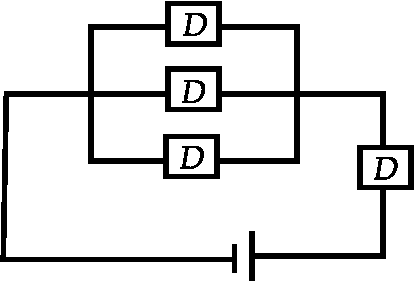
\includegraphics[height=2.5cm,width=4cm]{Net-19-19}
\end{figure}
The probability that a non-zero current flows through the circuit is
 \begin{tasks}(4)
	\task[\textbf{a.}] $2-p-p^{3}$
	\task[\textbf{b.}] $(1-p)^{4}$
	\task[\textbf{c.}] $(1-p)^{2} p^{2}$
	\task[\textbf{d.}] $(1-p)\left(1-p^{3}\right)$
\end{tasks}
\begin{answer}
	For non-zero current, one of the parallel device should be conducting.
	\begin{align*}
	\text { one separate device must be conducting with } P(I)&=p \text { and } P(C)=1-p \text {. }\\
	P(1)&=1-p^{3}\\
	\because p^{3} \text { is probability being insulator and }\left(1-p^{3}\right)& \text { being conductor. }\\
	P(2)&=1-p\\
\text{	Thus }P&=P(1) P(2)=\left(1-p^{3}\right)(1-p)
	\end{align*}
		So the correct answer is \textbf{Option (d)}
\end{answer}
\item The solution of the differential equation $x \frac{d y}{d x}+(1+x) y=e^{-x}$ with the boundary condition $y(x=1)=0$, is
 \begin{tasks}(4)
	\task[\textbf{a.}]$\frac{(x-1)}{x} e^{-x}$
	\task[\textbf{b.}] $\frac{(x-1)}{x^{2}} e^{-x}$
	\task[\textbf{c.}] $\frac{(1-x)}{x^{2}} e^{-x}$
	\task[\textbf{d.}] $(x-1)^{2} e^{-x}$
\end{tasks}
\begin{answer}
	\begin{align*}
	x \frac{d y}{d x}+(1+x) y&=e^{-x} \Rightarrow \frac{d y}{d x}+\frac{(1+x)}{x} y=\frac{e^{-x}}{x}\\
\text{	Let }p&=\frac{1+x}{x}\\
	I . F&=e^{\int p d x}=e^{\int\left(1+\frac{1}{x}\right) d x}=e^{x} \cdot e^{\ln x}=x e^{x} \\
	y \cdot x \cdot e^{x}&=\int \frac{e^{-x}}{x} \cdot x e^{x} d x+C \Rightarrow y \cdot x \cdot e^{x}=x+C \\
	&=y=0 \text { at } x=1 \quad \Rightarrow C=-1 \quad \Rightarrow y \cdot x \cdot e^{x}=x-1 \Rightarrow y=\left[\frac{x-1}{x}\right] e^{-x}
	\end{align*}
		So the correct answer is \textbf{Option (a)}
\end{answer}
\item The value of the definite integral $\int_{0}^{\pi} \frac{d \theta}{5+4 \cos \theta}$ is
 \begin{tasks}(4)
	\task[\textbf{a.}]$\frac{4 \pi}{3}$
	\task[\textbf{b.}] $\frac{2 \pi}{3}$
	\task[\textbf{c.}]$\pi$
	\task[\textbf{d.}]$\frac{\pi}{3}$ 
\end{tasks}
\begin{answer}
	\begin{align*}
	I&=\frac{1}{2} \int_{0}^{2 \pi} \frac{d \theta}{5+4 \cos \theta}
\text{	(even function)}\\
z&=e^{i \theta} \quad \text { unit circle; } \quad d \theta=\frac{d z}{i z} \quad \text { and } \cos \theta=\frac{1}{2}\left[z+\frac{1}{z}\right]\\
\Rightarrow I&=\frac{1}{2} \oint_{C} \frac{d z / i z}{5+4 \cdot \frac{1}{2}\left[z+\frac{1}{z}\right]}=\frac{1}{4} \oint \frac{d z / i}{z^{2}+\frac{5}{2} z+1}\\
\text{Roots for poles: }&\frac{-5}{4} \pm \frac{3}{4}=-2, \frac{-1}{2}
\text{and Root }-2\text{ is outside unit circle.}\\
\text{Residue at }z&=\frac{-1}{2}\text{ which is simple pole is} =\frac{1}{-\frac{1}{2}+2}=\frac{2}{3}\\
\text{Thus }I&=\frac{1}{4 i} \times 2 \pi i \times \frac{2}{3}=\frac{\pi}{3}.
	\end{align*}
		So the correct answer is \textbf{Option (d)}
\end{answer}
\item In a system comprising of approximately $10^{23}$ distinguishable particles, each particle may occupy any of 20 distinct states. The maximum value of the entropy per particle is nearest to
 \begin{tasks}(4)
	\task[\textbf{a.}] $20 k_{B}$
	\task[\textbf{b.}]$3 k_{B}$
	\task[\textbf{c.}]$10(\ln 2) k_{B}$
	\task[\textbf{d.}]$20(\ln 2) k_{B}$ 
\end{tasks}
\begin{answer}
	\begin{align*}
	\text { For } N \text { particles; } \omega&=20^{N} \text {. }\\
	S=k_{B} \ln \omega&=k_{B} \ln 20^{N}=N k_{B} \ln 20 \Rightarrow \frac{S}{N}=k_{B} \ln 20 \approx 3 k_{B} \quad \because \ln 20 \approx 3
	\end{align*}
		So the correct answer is \textbf{Option (b)}
\end{answer}
\item  Consider a classical gas in thermal equilibrium at temperatures $T_{1}$ and $T_{2}$ where $T_{1}<T_{2}$. Which of the following graphs correctly represents the qualitative behaviour of the probability density function of the $x$-component of the velocity?
 \begin{tasks}(2)
	\task[\textbf{a.}]
	\begin{figure}[H]
		\centering
		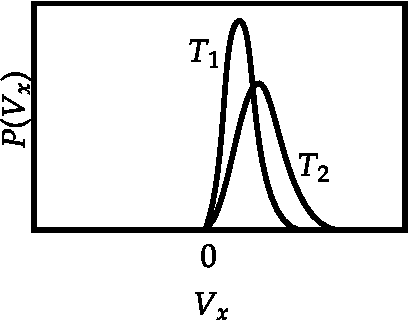
\includegraphics[height=2.5cm,width=3.5cm]{Net-19-20}
	\end{figure}
	\task[\textbf{b.}]
		\begin{figure}[H]
		\centering
		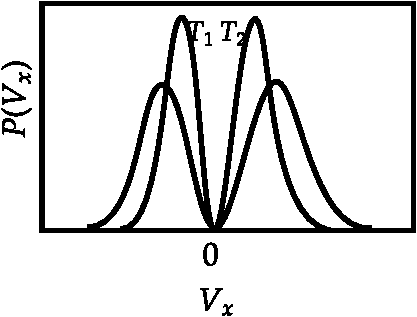
\includegraphics[height=2.5cm,width=3.5cm]{Net-19-21}
	\end{figure}
	\task[\textbf{c.}]
		\begin{figure}[H]
		\centering
		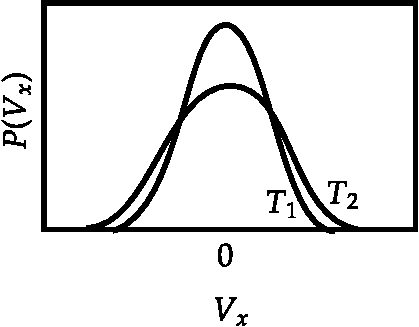
\includegraphics[height=2.5cm,width=3.5cm]{Net-19-22}
	\end{figure}
	\task[\textbf{d.}] 
		\begin{figure}[H]
		\centering
		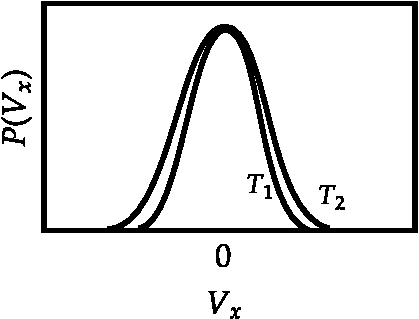
\includegraphics[height=2.5cm,width=3.5cm]{Net-19-23}
	\end{figure}
\end{tasks}
\begin{answer}$\left. \right. $\\
	\begin{figure}[H]
		\centering
		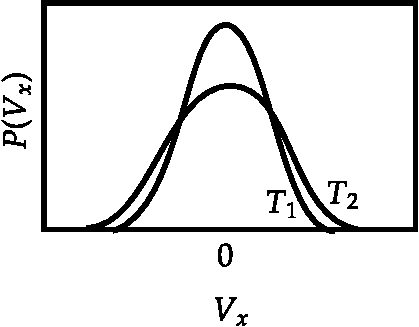
\includegraphics[height=2.5cm,width=3.5cm]{Net-19-22}
	\end{figure}
	\begin{align*}
	f\left(V_{x}\right)&=\left(\frac{m}{2 \pi k T}\right)^{1 / 2} e^{-\frac{m V_{x}^{2}}{2 k T}} \text { where }-\infty<V_{x}<\infty\\
	\text { and }\left\langle V_{x}>=0,<V_{x}^{2}\right\rangle&=\frac{k T}{m}, V_{x, r m s}=\sqrt{\frac{k T}{m}} \text {. }\\
	\text{So mean value remains same }&\text{and r.m.s shift towards right}\\
	\text{or left hence area under}&\text{ the curve is same. Thus distribution is broad.}
	\end{align*}
		So the correct answer is \textbf{Option (c)}
\end{answer}
\item  The equation of state of an ideal gas is $p V=R T .$ At very low temperatures, the volume expansion coefficient $\frac{1}{V} \frac{\partial V}{\partial T}$ at constant pressure
 \begin{tasks}(2)
	\task[\textbf{a.}]Diverges as $\frac{1}{T^{2}}$
	\task[\textbf{b.}]Diverges as $\frac{1}{T}$
	\task[\textbf{c.}]Vanishes as $T$
	\task[\textbf{d.}]Is independent of the temperature 
\end{tasks}
\begin{answer}
	\begin{align*}
	p V&=R T \Rightarrow V=\frac{R T}{p}\\
	\alpha&=\frac{1}{V} \cdot \frac{d V}{d T}=\frac{1}{V} \cdot \frac{R}{p} \Rightarrow \alpha=\frac{R}{R T}=\frac{1}{T}\\
	\text{As }T &\rightarrow 0, \alpha \rightarrow \infty.
	\end{align*}
		So the correct answer is \textbf{Option (b)}
\end{answer}
\item  The Hamiltonian of a classical nonlinear one dimensional oscillator is $H=\frac{1}{2 m} p^{2}+\lambda x^{4}$, where $\lambda>0$ is a constant. The specific heat of a collection of a collection of $N$ independent such oscillators is
 \begin{tasks}(4)
	\task[\textbf{a.}]$\frac{3 N k_{B}}{2}$
	\task[\textbf{b.}]$\frac{3 N k_{B}}{4}$
	\task[\textbf{c.}]$N k_{B}$
	\task[\textbf{d.}]$\frac{N k_{B}}{2}$ 
\end{tasks}
\begin{answer}
	\begin{align*}
	H&=\frac{p^{2}}{2 m}+\lambda x^{4}, \quad \lambda>0\\
	\langle H\rangle&=\left\langle\frac{p^{2}}{2 m}\right\rangle+\langle V\rangle=\frac{1}{2} k_{B} T+2 \lambda \frac{\int_{0}^{\infty} x^{4} e^{-\beta \lambda x^{4}} d x}{2 \int_{0}^{\infty} e^{-\beta x^{4}} d x}=\frac{1}{2} k_{B} T+2 \lambda \frac{\frac{\sqrt{5 / 4}}{4(\lambda \beta)^{5 / 4}}}{2 \frac{\sqrt{5 / 4}}{(\lambda \beta)^{1 / 4}}}\\
	\Rightarrow\langle H\rangle&=\frac{1}{2} k_{B} T+\lambda \frac{(\lambda \beta)^{1 / 4}}{4(\lambda \beta)^{5 / 4}}=\frac{1}{2} k_{B} T+\frac{\lambda}{4} \frac{1}{\lambda \beta}=\frac{1}{2} k_{B} T+\frac{k_{B} T}{4}=\frac{3}{4} k_{B} T=\frac{3}{4} k_{B} T \\
	\Rightarrow C_{V}&=\frac{3}{4} N k_{B}
	\end{align*}
		So the correct answer is \textbf{Option (b)}
\end{answer}
\item  In an experiment to measure the acceleration due to gravity $g$ using a simple pendulum, the length and time period of the pendulum are measured to three significant figures. The mean value of $g$ and the uncertainty $\delta g$ of the measurements are then estimated using a calculator from a large number of measurements and found to be $9.82147 \mathrm{~m} / \mathrm{s}^{2}$ and $0.02357 \mathrm{~m} / \mathrm{s}^{2}$, respectively. Which of the following is the most accurate way of presenting the experimentally determined value of $g$ ?
 \begin{tasks}(2)
	\task[\textbf{a.}]$9.82 \pm 0.02 \mathrm{~m} / \mathrm{s}^{2}$
	\task[\textbf{b.}]$9.8215 \pm 0.02 \mathrm{~m} / \mathrm{s}^{2}$
	\task[\textbf{c.}]$9.82147 \pm 0.02357 \mathrm{~m} / \mathrm{s}^{2}$
	\task[\textbf{d.}] $9.82 \pm 0.02357 \mathrm{~m} / \mathrm{s}^{2}$ 
\end{tasks}
\begin{answer}
	So the correct answer is \textbf{Option (d)}
\end{answer}
\item  An ac signal of the type as shown in the figure, is applied across a resistor $R=1 \Omega$.
\begin{figure}[H]
	\centering
	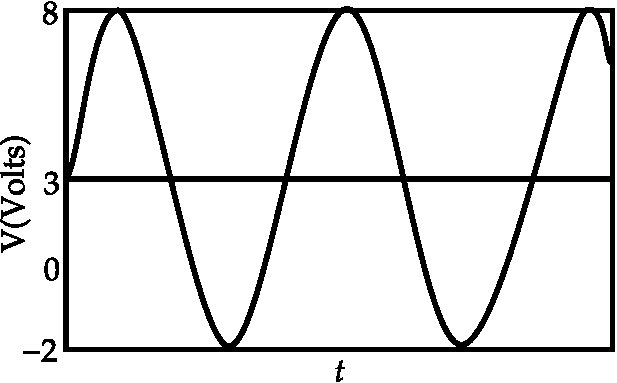
\includegraphics[height=2.5cm,width=4cm]{Net-19-24}
\end{figure}
The power dissipated across the resistor is
 \begin{tasks}(4)
	\task[\textbf{a.}]$12.5 \mathrm{~W}$
	\task[\textbf{b.}]$9 \mathrm{~W}$
	\task[\textbf{c.}]$25 \mathrm{~W}$
	\task[\textbf{d.}]$21.5 \mathrm{~W}$ 
\end{tasks}
\begin{answer}
	\begin{align*}
	\text { Peak value } V_{m}&=5 V, V_{m s}=\frac{V_{m}}{\sqrt{2}}\\
	\text{Power dissipated }P_{a c}&=\frac{V_{r m s}^{2}}{R}=\frac{V_{m}^{2}}{2 R}=\frac{25}{2 \times 1}=12.5 \mathrm{~W}\\
	P_{d c}&=\frac{V^{2}}{R}=\frac{(3)^{2}}{1}=9.0 \mathrm{~W}\\
	\text{Total power dissipated }P&=P_{a c}+P_{d c}=12.5 \mathrm{~W}+9.0 \mathrm{~W}=21.5 \mathrm{~W}
	\end{align*}
		So the correct answer is \textbf{Option (d)}
\end{answer}
\item  An npn-transistor is connected in a voltage divider configuration as shown in the figure below.
\begin{figure}[H]
	\centering
	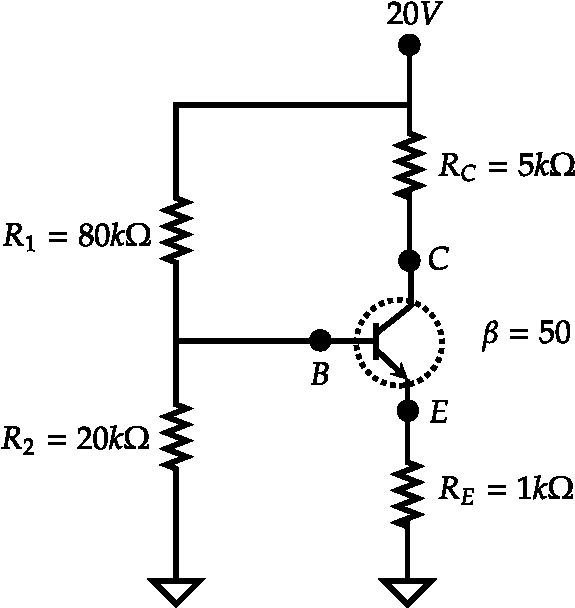
\includegraphics[height=4.3cm,width=4cm]{Net-19-25}
\end{figure}
If the resistor $R_{2}$ is disconnected, the voltages $V_{B}$ at the base and $V_{C}$ at the collector change as follows.
 \begin{tasks}(2)
	\task[\textbf{a.}]Both $V_{B}$ and $V_{C}$ increase
	\task[\textbf{b.}]Both $V_{B}$ and $V_{C}$ decrease
	\task[\textbf{c.}]$V_{B}$ decreases, but $V_{C}$ increases
	\task[\textbf{d.}]$V_{B}$ increases, but $V_{C}$ decreases
\end{tasks}
\begin{answer}
	\begin{align*}
	V_{B}&=\frac{V_{C C} R_{2}}{R_{1}+R_{2}}=\frac{V_{C C}}{R_{1} / R_{2}+1} \quad \text { as } R_{2} \uparrow, V_{B} \uparrow\\
	\because V_{E}&=V_{B}-V_{B E} \text { and } I_{E}=\frac{V_{E}}{R_{E}} \approx I_{C} \\
	\quad& \text { As } V_{B} \uparrow, V_{E} \uparrow \text { thus } I_{E} \approx I_{C} \uparrow \\
	\because V_{C C}&=V_{C C}-I_{C} R_{C}, \quad \text { as } I_{C} \uparrow, V_{C} \downarrow
	\end{align*}
		So the correct answer is \textbf{Option (d)}
\end{answer}
\item  Let $Y$ denote the output in the following logical Circuit.
\begin{figure}[H]
	\centering
	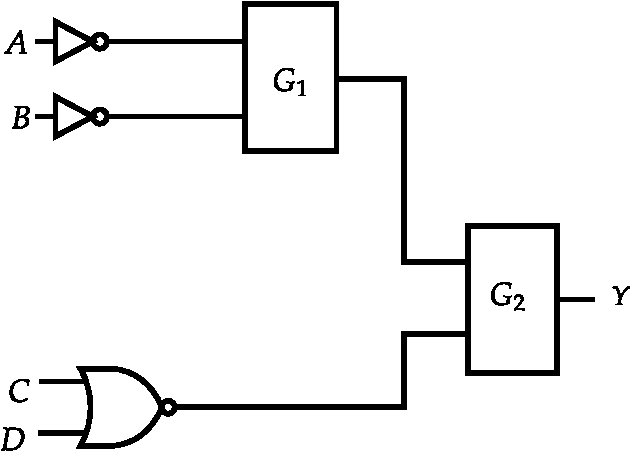
\includegraphics[height=3cm,width=4.5cm]{Net-19-26}
\end{figure}
If $Y=A B+\overline{C D}$, the gates $G_{1}$ and $G_{2}$ must, respectively, be
 \begin{tasks}(2)
	\task[\textbf{a.}]OR and NAND
	\task[\textbf{b.}]NOR and $\mathrm{OR}$
	\task[\textbf{c.}] AND and NAND
	\task[\textbf{d.}]  NAND and OR
\end{tasks}
\begin{answer}
	\begin{align*}
	\text{1. }&Y=\overline{(\bar{A}+\bar{B})+(\overline{C+D})}=\overline{(\bar{A}+\bar{B})}+\overline{(\overline{C+D})}=A B+C D\\
		\text{2. }&Y=\overline{(\bar{A}+\bar{B})}+(\overline{C+D})=A B+\bar{C} \bar{D}\\
		\text{3. }&Y=\overline{(\bar{A}+\bar{B})+(\overline{C+D})}=\overline{\bar{A} \bar{B}}+\overline{(\overline{C+D})}=(A+B)+(C+D)\\
		\text{4. }&Y=\overline{\bar{A} \bar{B}}+(\overline{C+D})=A+B+\bar{C} \bar{D}
	\end{align*}
		So the correct answer is \textbf{Option (b)}
\end{answer}
\item  A solid spherical Cork of radius $R$ and specific gravity $0.5$ floats on water. The cork is pushed down so that its Centre of mass is at a distance $h$ (where $0<h<R$ ) below the surface of water, and Then released. The volume of the part of the cork above water level is $\pi R^{3}\left(\frac{2}{3}-\cos \theta_{0}+\frac{1}{3} \cos ^{3} \theta_{0}\right)$ where $\theta_{0}$ is the angle as shown in the figure.
\begin{figure}[H]
	\centering
	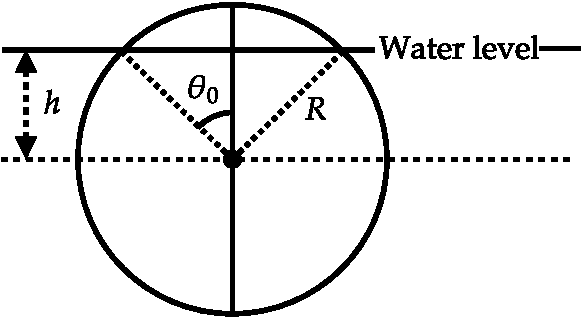
\includegraphics[height=2.7cm,width=5cm]{Net-19-27}
\end{figure}
At the moment of release, the dependence of the upward force on the cork on $h$ is
 \begin{tasks}(4)
	\task[\textbf{a.}]$\frac{h}{R}-\frac{1}{3}\left(\frac{h}{R}\right)^{3}$
	\task[\textbf{b.}]$\frac{h}{R}+\frac{1}{3}\left(\frac{h}{R}\right)^{3}$
	\task[\textbf{c.}]$\frac{h}{R}-\frac{2}{3}\left(\frac{h}{R}\right)^{3}$
	\task[\textbf{d.}] $\frac{h}{R}+\frac{2}{3}\left(\frac{h}{R}\right)^{3}$
\end{tasks}
\begin{answer}
	\begin{align*}
	\text { volume of sphere }&=\frac{4 \pi}{3} R^{3}\\
	\text { Weight of sphere }&=\frac{4 \pi}{3} R^{3} g \times 0.5 \Rightarrow F_{W}=\frac{2 \pi}{3} R^{3} g \text { in down ward direction }\\
\text { volume of liquid }&\text{displaces by cork }\\
\frac{4 \pi R^{3}}{3}-\pi R^{3}\left[\frac{2}{3}-\cos \theta_{0}+\frac{1}{3} \cos ^{3} \theta_{0}\right]&=\frac{2 \pi R^{3}}{3}+\pi R^{3} \cos \theta_{0}-\frac{\pi R^{3}}{3} \cos ^{3} \theta_{0} \quad \cos \theta_{0}=\frac{h}{R}\\
V_{1}&=\frac{2 \pi R^{3}}{3}+\left(\frac{h}{R}-\frac{1}{3}\left(\frac{h}{R}\right)^{3}\right) \pi R^{3}\\
\text { weight at displaced liquid }& V_{1} d g \text { where } d=1\\
F_{B}&=\frac{2 \pi R^{3}}{3} g+\left[\frac{h}{R}-\frac{1}{3}\left(\frac{h}{R}\right)^{3}\right] g \pi R^{3} \\\Rightarrow \Delta F&=F_{B}-F_{W}=\left[\frac{h}{R}-\frac{1}{3}\left(\frac{h}{R}\right)^{3}\right] \pi R^{3} \\
\Delta F &\propto \frac{h}{R}-\frac{1}{3}\left(\frac{h}{R}\right)^{3}
	\end{align*}
		So the correct answer is \textbf{Option (a)}
\end{answer}
\item Two particles of masses $m_{1}$ and $m_{2}$ are connected by a massless thread of length $l$ as shown in figure below.
\begin{figure}[H]
	\centering
	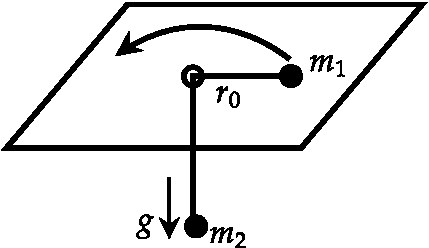
\includegraphics[height=2cm,width=4cm]{Net-19-28}
\end{figure}
The particle of mass in on the plane undergoes a circular motion with radius $r_{0}$ and angular momentum $L$. When a small radial displacement $\in$ (whew $\in<<r_{0}$ ) is applied, its radial coordinate is found to oscillate about $r_{0}$. The frequency of the oscillations is
 \begin{tasks}(4)
	\task[\textbf{a.}] $\sqrt{\frac{7 m_{2} g}{\left(m_{1}+\frac{m_{2}}{2}\right) r_{0}}}$
	\task[\textbf{b.}]$\sqrt{\frac{7 m_{2} g}{\left(m_{1}+m_{2}\right) r_{0}}}$
	\task[\textbf{c.}]$\sqrt{\frac{3 m_{2} g}{\left(m_{1}+\frac{m_{2}}{2}\right) r_{0}}}$
	\task[\textbf{d.}] $\sqrt{\frac{3 m_{2} g}{\left(m_{1}+m_{2}\right) r_{0}}}$
\end{tasks}
\begin{answer}
	\begin{align*}
	L=\frac{1}{2}\left(m_{1}+m_{2}\right) \ddot{r}+&\frac{1}{2} m_{1} r^{2} \dot{\theta}^{2}-m_{2} g(l-r)\\
\text{	Lagrangian equation of motion; }&
	\frac{d}{d t}\left(\frac{\partial L}{\partial \dot{r}}\right)-\frac{\partial L}{\partial r}=0\\
	\left(m_{1}+m_{2}\right) \ddot{r}-m_{1} r \dot{\theta}^{2}+m_{2} g&=0\\
	\text{Hence angular momentum}&\text{  is conserved}\\
	m_{1} r^{2} \dot{\theta}&=m_{1} r_{0}^{2} \dot{\theta}_{0} \Rightarrow \dot{\theta}=\frac{r_{0}^{2} \dot{\theta}_{0}}{r^{2}}\\
	\text { For circular motion } m r_{0} \dot{\theta}_{0}^{2}&=m_{2} g\\
	\text { so } r \dot{\theta}^{2}&=\frac{m_{2}}{m_{1}}\left(\frac{r_{0}}{r}\right)^{3} g \\
	\left(m_{1}+m_{2}\right) \ddot{r}-m_{2}\left(\frac{r_{0}}{r}\right)^{3} g+m_{2} g&=0\\
\text{	Put }r&=r_{0}+\in \ddot{r}=\ddot{\in}\\
	\left(m_{1}+m_{2}\right) \ddot{\in}&-m_{2}\left(\frac{r_{0}}{r_{0}+\epsilon}\right)^{3} g+m_{2} g \\
	\Rightarrow\left(m_{1}+m_{2}\right)& \ddot{\in}-m_{2} r_{0}^{3}\left(r_{0}+\epsilon\right)^{-3} g+m_{2} g \\
	\left(m_{1}+m_{2}\right) \ddot{\in}&-m_{2} r_{0}^{3} g r_{0}^{-3}\left(1+\frac{\epsilon}{r_{0}}\right)^{-3}+m_{2} g=0 \\
	\left(m_{1}+m_{2}\right) \ddot{\in}&+\frac{m_{2} 3 \in}{r_{0}}=0 \Rightarrow \omega=\sqrt{\frac{3 m_{2} g}{\left(m_{1}+m_{2}\right) r_{0}}}
	\end{align*}
	So the correct answer is \textbf{Option (d)}
\end{answer}
\item  The time evolution of a coordinate $x$ of a particle is described by the equation
$$
\frac{d^{2} x}{d t^{4}}+2 \Omega^{2} \frac{d^{2} x}{d t^{2}}+\left(\Omega^{4}-A^{4}\right) x=0
$$
For $\Omega>A$, the particle will
 \begin{tasks}(1)
	\task[\textbf{a.}]Eventually come to rest at the origin
	\task[\textbf{b.}] Eventually drift to infinity $(|x| \rightarrow \infty)$
	\task[\textbf{c.}] Oscillate about the origin
	\task[\textbf{d.}] Eventually come to rest at $\frac{\Omega}{A}$ or $-\frac{\Omega}{A}$
\end{tasks}
\begin{answer}
	\begin{align*}
\text{	Let }x&=e^{k t}
\text{	(degree is one)}\\
k^{4}&+2 \Omega^{2} k^{2}+\left(\Omega^{4}-A^{4}\right)=0 \\
\text { Put } k^{2}&=u \Rightarrow u^{2}+2 \Omega^{2} u+\left(\Omega^{4}-A^{4}\right)=0 \\
u&=-\Omega^{2} \pm A^{2} \\
u&=-\Omega^{2}-A^{2},-\Omega^{2}+A^{2} \\
u&=-\left(\Omega^{2}+A^{2}\right),-\left(\Omega^{2}-A^{2}\right) \\
k^{2}&=-\left(\Omega^{2}+A^{2}\right), k^{2}=-\left(\Omega^{2}-A^{2}\right)\\
k&=\pm i \sqrt{\Omega^{2}+A^{2}}, k=\pm i \sqrt{\Omega^{2}-A^{2}} ; \quad \Omega>A\\
&\text{So, oscillatory about the origin}
	\end{align*}
		So the correct answer is \textbf{Option (c)}
\end{answer}
\item  The Hamiltonian of a quantum particle of mass $m$ is $H=\frac{p^{2}}{2 m}+\alpha|x|^{r}$, where $\alpha$ and $r$ are positive constants. The energy $E_{n}$ of the $n^{t h}$ level for large $n$, depends on $n$ as
 \begin{tasks}(4)
	\task[\textbf{a.}]$n^{2 r}$
	\task[\textbf{b.}]$n^{r+2}$
	\task[\textbf{c.}]$n^{1 /(r+2)}$
	\task[\textbf{d.}] $n^{2 r /(r+2)}$
\end{tasks}
\begin{answer}
	\begin{align*}
	\text{According to Bohr }&\text{Summerfield theorem,}\\
	E&=\frac{P_{x}^{2}}{2 m}+\alpha|x|^{r} \text {. Thus if } P_{x}=0 \Rightarrow x=\pm\left(\frac{E}{\alpha}\right)^{1 / r}\\
	\oint P_{x} d x&=n h \Rightarrow \oint \sqrt{2 m\left(E-\alpha|x|^{r}\right)} d x=n h \quad \Rightarrow 4 \int_{0}^{\left(\frac{E}{\alpha}\right)^{1 / r}} \sqrt{2 m\left(E-\alpha x^{r}\right)} d x=n h\\
	&4 \times \sqrt{2 m E} \times\left(\frac{E}{\alpha}\right)^{1 / r} \int_{0}^{1} \sqrt{1-t^{r}} d t=n h\\
	&E^{1 / 2} E^{1 / r} \propto n \Rightarrow E^{\frac{r+2}{2 r}} \propto n \quad \Rightarrow E \propto n^{\frac{2 r}{r+2}}
	\end{align*}
	So the correct answer is \textbf{Option (d)}
\end{answer}
\item In the partial wave expansion, the differential scattering cross-section is given by
$$
\frac{d \sigma}{d(\cos \theta)}=\left|\sum_{l}(2 l+1) e^{i \delta_{i}} \sin \delta_{l} P_{l}(\cos \theta)\right|^{2}
$$
where $\theta$ is the scattering angle. For a certain neutron-nucleus scattering. It is found that the two lowest phase shifts $\delta_{0}$ and $\delta_{1}$ corresponding to $s$-wave and $p$-wave, respectively, satisfy $\delta_{1} \approx \frac{\delta_{0}}{2}$. Assuming that the other phase shifts are negligibly small, the differential cross-section reaches its minimum for $\cos \theta$ equal to
 \begin{tasks}(4)
	\task[\textbf{a.}]0
	\task[\textbf{b.}] $\pm 1$
	\task[\textbf{c.}]$-\frac{2}{3} \cos ^{2} \delta_{1}$
	\task[\textbf{d.}]  $\frac{1}{3} \cos ^{2} \delta_{1}$
\end{tasks}
\begin{answer}
	\begin{align*}
	D(\theta)&=\sum_{l}(2 l+1) e^{i \delta l} \sin \delta_{l} P_{l}(\cos \theta)\\
	l&=0,1 \quad\text{ Let }l_{1}=0,1 \quad l_{2}=0,1\\
	D(\theta)&=\left(\sum_{l_{1}}\left(2 l_{1}+1\right) e^{i \delta_{l_{1}}} \sin \delta_{l_{1}} P_{l_{1}}(\cos \theta)\right)\left(\sum_{l_{2}}\left(2 l_{2}+1\right) e^{-i \delta_{1}} \sin \delta_{l_{2}} P_{l_{2}}(\cos \theta)\right)\\
	\text{Put }l_{1}&=0,1 \quad\text{ Put }l_{2}=0,1\\
	D(\theta)=& {\left[e^{i \delta_{0}} \sin \delta_{0} p_{0}(\cos \theta)\right]\left[e^{-i \delta_{0}} \sin \delta_{0} p_{0}(\cos \theta)\right]+} \\
	& {\left[3 e^{i \delta_{1}} \sin \delta_{1} p_{1}(\cos \theta)\right]\left[3 e^{-i \delta_{1}} \sin \delta_{1} p_{1}(\cos \theta)\right]+} \\
	& {\left[e^{i \delta_{0}} \sin \delta_{0} p_{0}(\cos \theta)\right]\left[3 e^{-i \delta_{1}} \sin \delta_{1} p_{1}(\cos \theta)\right]+} \\
	& {\left[3 e^{i \delta_{1}} \sin \delta_{1} p_{1}(\cos \theta)\right]\left[e^{-i \delta_{0}} \sin \delta_{0} p_{0}(\cos \theta)\right] }\\
	D(\theta)&=\sin ^{2} \delta_{0}+9 \sin ^{2} \frac{\delta_{0}}{2} \cos ^{2} \theta+\frac{3}{2} \sin ^{2} \delta_{0} \cos \theta\left[e^{i \delta_{0}} e^{-i \delta_{1}}+e^{i \delta_{1}} e^{-i \delta_{0}}\right] \\
	D(\theta)&=\sin ^{2} \delta_{0}+9 \sin ^{2} \delta_{1} \cos ^{2} \theta+3 \sin \delta_{0} \sin \delta_{1} P_{1}(\cos \theta)\left[e^{i \delta_{0}} e^{-i \delta_{1}}+e^{i \delta_{1}} e^{-i \delta_{0}}\right] \\
	\left(\frac{d D}{d \theta}\right)&=018 \sin ^{2} \frac{\delta_{0}}{2}(-\sin \theta \cos \theta)+\frac{3}{2} \sin ^{2} \delta_{0}(-\sin \theta)=0 \\
	\sin \theta&=0, \cos \theta=\pm 1\\
	\cos \theta \sin ^{2} \frac{\delta_{0}}{2}+\frac{3}{2} \sin ^{2} \delta_{0}&=0 \cos \theta=\frac{-2}{3} \cos ^{2} \frac{\delta_{0}}{2}=\frac{-2}{3} \cos ^{2} \delta_{1}
	\end{align*}
		So the correct answer is \textbf{Option (c)}
\end{answer}
\item A charged, spin-less particle of mass $m$ is subjected to an attractive potential $V(x, y, z)=\frac{1}{2} k\left(x^{2}+y^{2}+z^{2}\right)$, where $k$ is a positive constant. Now a perturbation in the form of a weak magnetic field $B=B_{0} \hat{k}$ (where $B_{0}$ is a constant) is switched on. Into how many distinct levels will the second excited state of the unperturbed Hamiltonian split?
 \begin{tasks}(4)
	\task[\textbf{a.}]5
	\task[\textbf{b.}]4
	\task[\textbf{c.}]2
	\task[\textbf{d.}] 1
\end{tasks}
\begin{answer}
	\begin{align*}
	B&=B_{0} \hat{k}\\
	\text{We can choose}&\text{ vector potential}\\
	A_{\rho}&=0, A_{z}=0 A_{\varphi}=\frac{1}{2} B_{0} \rho \\
	H&=\frac{1}{2 m}\left[\vec{P}-\frac{q \vec{A}}{c}\right]^{2}+V=\frac{1}{2} \frac{P_{e}^{2}}{m}-\frac{q}{m c} \vec{P} \cdot \vec{A}+\frac{q^{2}}{2 m c^{2}} A^{2}+\frac{1}{2} k P^{2}+\frac{1}{2} k z^{2} \\
	\vec{\Delta} \cdot \vec{A}&=0 \vec{P} \cdot \vec{A}=\vec{A} \cdot \vec{P} \\
	&=\frac{P^{2} e}{2 m}+\frac{1}{2} m \omega_{1}^{2} \rho^{2}+\left(\frac{P_{2}^{2}}{2 m}+\frac{1}{2} k z^{2}\right)-\frac{Q B_{0}}{2 m c} \vec{L}_{2}\\
	\text{where }\vec{L}_{2}&=\hat{P}_{2} \rho\hspace{1cm}
	\omega_{0}=\frac{Q B}{2 m c}\\
	\text{We write our Hamiltonian  }&\text{in cylindrical co-ordinate}\\
	E_{n_{e}, n_{z}, m}&=E_{\left(n_{x}, n_{y}\right), n_{z}, m}\\
	n_{\rho}&=0,1,2,3 \ldots \\
	n_{z}&=0,1,2,3 \ldots \\
	E&=\left(n_{x}+n_{y}+1\right) \hbar \omega_{1}+\left(n_{2}+\frac{1}{2}\right) \hbar \omega_{2}+m \hbar \omega_{0}
	\end{align*}
	\begin{align*}
	\renewcommand*{\arraystretch}{1.5}
	\begin{array}{lll}
E_{(2,0,0)}+\omega_{0} \hbar \quad E_{0,2,0}+\omega_{0} \hbar\qquad &\longrightarrow \qquad &\text { (i) Same energy level }\\
E_{(2,0,0)}-\omega_{0} \hbar \quad E_{0,2,0}-\omega_{0} \hbar \qquad &\longrightarrow \qquad & \text { (ii) Energy level }\\
E_{1,1,0}+\omega_{0} \hbar \qquad &\longrightarrow \qquad &\text { (ii) Energy level }\\
E_{110}-\omega_{0} \hbar \qquad &\longrightarrow \qquad &\text { (ii) Energy level }
	\end{array}\\
	\text { so it splits into (iv) level }
	\end{align*}
		So the correct answer is \textbf{Option (a)}
\end{answer}
\item  The elastic scattering of a charged particle of mass $m$ off an atom can be approximated by the potential $V(r)=\frac{\alpha}{r} e^{-r / R}$ where $\alpha$ and $R$ are positive constants.\\
If the wave number of the incoming particle is $k$ and the scattering angle is $2 \theta$, the differential cross-section in the Born approximation is
 \begin{tasks}(2)
	\task[\textbf{a.}]$\frac{m^{2} \alpha^{2} R^{4}}{4 \hbar^{4}\left(1+k^{3} R^{2} \sin ^{2} \theta\right)}$
	\task[\textbf{b.}]$\frac{m^{2} \alpha^{2} R^{4}}{\hbar^{4}\left(2 k^{2} R^{2} \sin ^{2} \theta\right)^{2}}$
	\task[\textbf{c.}] $\frac{2 m^{2} \alpha^{2} R^{4}}{\hbar^{4}\left(2 k^{2} R^{2} 2 \sin ^{2} \theta\right)}$
	\task[\textbf{d.}] $\frac{4 m^{2} \alpha^{2} R^{4}}{\hbar^{4}\left(1+4 k^{2} R^{2} \sin ^{2} \theta\right)^{2}}$
\end{tasks}
\begin{answer}
	\begin{align*}
	V(r)&=\frac{\alpha}{r} e^{-r / R}\\
	f(\theta)&=\frac{-2 m}{\hbar^{2} q} \int_{0}^{\infty} r V(r) \sin q r d r\\
	q&=2 k \sin \theta \quad \text { where } 2 \theta \text { is scattering angle } D(\theta)=|f(\theta)|^{2}\\
	f(\theta)&=\frac{-2 m}{\hbar^{2} q} \int_{0}^{\infty} r \frac{\alpha}{r} e^{-r / R} \sin q r d r\\
	\text{put }\sin q r&=\frac{e^{i q r}-e^{-i q r}}{2 i}\\
	f(\theta)&=\frac{-2 m \alpha}{\hbar^{2}\left[\frac{1}{R^{2}}+q^{2}\right]}\\
	D(\theta)&=\frac{4 m^{2} \alpha^{2}}{\hbar^{2}\left[\frac{1}{R^{2}}+(2 k \sin \theta)^{2}\right]^{2}}=\frac{4 m^{2} \alpha^{2} R^{2}}{\hbar^{4}\left[1+4 R^{2} k^{2} \sin ^{2} \theta\right]^{2}}
	\end{align*}
		So the correct answer is \textbf{Option (d)}
\end{answer}
\item  The wave number $k$ and the angular frequency $\omega$ of a wave are related by the dispersion relation $\omega^{2}=\alpha k+\beta k^{3}$ where $\alpha$ and $\beta$ are positive constants. The wave number for which the phase velocity equals the group velocity, is
 \begin{tasks}(4)
	\task[\textbf{a.}]$3 \sqrt{\frac{\alpha}{\beta}}$
	\task[\textbf{b.}]$\sqrt{\frac{\alpha}{\beta}}$
	\task[\textbf{c.}]$\frac{1}{2} \sqrt{\frac{\alpha}{\beta}}$
	\task[\textbf{d.}] $\frac{1}{3} \sqrt{\frac{\alpha}{\beta}}$
\end{tasks}
\begin{answer}
	\begin{align*}
	\omega^{2}&=\alpha k+\beta k^{3}\\
	2 \omega \frac{d \omega}{d k}&=\alpha+3 \beta k^{2} \Rightarrow \frac{d \omega}{d k}=\frac{\alpha+3 \beta k^{2}}{2 \omega}\\
\text{	also }\omega \cdot \frac{\omega}{k}&=\alpha+\beta k^{2}\\
\text { divide (1) and (2) }&\\
\frac{d \omega / d k}{\omega(\omega / k)}&=\frac{\alpha+3 \beta k^{2}}{2 \omega} \times \frac{1}{\alpha+\beta k^{2}} \\
\because \frac{d \omega}{d k}&=\frac{\omega}{k}\\
\Rightarrow 2 \alpha+2 \beta k^{2}&=\alpha+3 \beta k^{2} \Rightarrow \alpha=\beta k^{2} \Rightarrow k=\sqrt{\frac{\alpha}{\beta}}
	\end{align*}
		So the correct answer is \textbf{Option (b)}
\end{answer}
\item  A inertial observer $A$ at rest measures the electric and magnetic field $E=(\alpha, 0,0)$ and $B=(\alpha, 0,2 \alpha)$ in a region, where a is a constant. Another inertial observer $B$, moving with a constant velocity with respect to $A$, measures the fields as $E^{\prime}=\left(E_{x}^{\prime}, \alpha, 0\right)$ and $B^{\prime}=\left(\alpha, B_{y}^{\prime}, \alpha\right)$. Then in units $c=1, E_{x}^{\prime}$ and $B_{y}^{\prime}$ are given, respectively, by
 \begin{tasks}(4)
	\task[\textbf{a.}]$-2 \alpha$ and $\alpha$
	\task[\textbf{b.}] $2 \alpha$ and $-\alpha$
	\task[\textbf{c.}] $\alpha$ and $-2 \alpha$
	\task[\textbf{d.}] $-\alpha$ and $2 \alpha$
\end{tasks}
\begin{answer}
	\begin{align*}
	\text { From } S&\\
	\vec{E} \cdot \vec{B} &\text { is invariant and } E^{2}-B^{2} \text { is invariant }\\
	E_{x}^{\prime} \alpha+B_{y}^{\prime} \alpha&=\alpha^{2} \Rightarrow E_{x}^{\prime}+B_{y}^{\prime}=\alpha \\
	E_{x}^{\prime 2}+\alpha^{2}-\left(B_{y}^{\prime 2}+\alpha^{2}+\alpha^{2}\right)&=+\alpha^{2}-\left(+\alpha^{2}+4 \alpha^{2}\right) \Rightarrow E_{x}^{\prime 2}-B_{y}^{\prime 2}=-3 \alpha^{2}\\
	\text { (Solving these two equation) }&\\
	E_{x}^{\prime}&=-\alpha, \quad B_{y}^{\prime}=2 \alpha
	\end{align*}
		So the correct answer is \textbf{Option (d)}
\end{answer}
\item  A point charge is moving with a uniform velocity $\beta C$ along the positive $x$-direction, parallel to and very close to a corrugated metal sheet (see the figure below).
\begin{figure}[H]
	\centering
	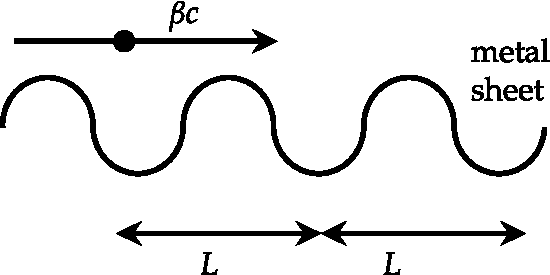
\includegraphics[height=2.5cm,width=4.5cm]{Net-19-29}
\end{figure}
The wavelength of the electromagnetic radiation received by an observer along the direction of motion is
 \begin{tasks}(4)
	\task[\textbf{a.}]$\frac{1}{\beta} \sqrt{1-\beta^{2}}$
	\task[\textbf{b.}]$L \sqrt{1-\beta^{2}}$
	\task[\textbf{c.}]$L \beta \sqrt{1-\beta^{2}}$
	\task[\textbf{d.}] $L$
\end{tasks}
\begin{answer}
	\begin{align*}
	\intertext{ Assume the wavelength at radiation if choose is rest with respect to observe $=\lambda_{0}=L$ From Doppler effect if relation move towards observe}
	\lambda&=L \sqrt{\frac{1-\beta}{1+\beta}} \sqrt{\frac{1+\beta}{1+\beta}} \Rightarrow \lambda=L \sqrt{\frac{(1-\beta)(1+\beta)}{(1+\beta)(1+\beta)}} \\
	\Rightarrow \lambda&=\frac{L}{1+\beta} \sqrt{1-\beta^{2}} \Rightarrow \lambda \simeq \frac{1}{\beta} \sqrt{1-\beta^{2}} \qquad 1+\beta \simeq \beta
	\end{align*}
	So the correct answer is \textbf{Option (a)}
\end{answer}
\item If the Newton-Raphson method is used to find the positive root of the equation $x=2 \sin x$, the iteration equation is
 \begin{tasks}(2)
	\task[\textbf{a.}]$x_{n+1}=\frac{2 x_{n}-2\left(\sin x_{n}+x_{n} \cos x_{n}\right)}{1-2 \cos x_{n}}$
	\task[\textbf{b.}]$x_{n+1}=\frac{2\left(\sin x_{n}-x_{n} \cos x_{n}\right)}{1-2 \cos x_{n}}$
	\task[\textbf{c.}] $x_{n+1}=\frac{x_{n}^{2}-1+2\left(\cos x_{n}-x_{n} \sin x_{n}\right)}{x_{n}-2 \sin x_{n}}$
	\task[\textbf{d.}]  $x_{n+1}=\frac{x_{n}^{2}-1-2\left(\cos x_{n}+\sin x_{n}\right)}{x_{n}-2 \sin x_{n}}$
\end{tasks}
\begin{answer}
	\begin{align*}
	f(x)&=x-2 \sin x \Rightarrow f^{\prime}(x)=1-2 \cos x\\
	x_{n+1} &=x_{n}-\frac{f(x)}{f^{\prime}(x)} \\
	x_{n+1} &=x_{n}-\frac{\left(x_{n}-2 \sin x_{n}\right)}{1-2 \cos x_{n}}=\frac{x_{n}-2 x_{n} \cos x_{n}-x_{n}+2 \sin x_{n}}{1-2 \cos x_{n}} \\
	x_{n+1} &=\frac{2\left[\sin x_{n}-x_{n} \cos x_{n}\right]}{1-2 \cos x_{n}}
	\end{align*}
\end{answer}
\item  The equation of motion of a forced simple harmonic oscillator is $\ddot{x}+\omega^{2} x=A \cos \Omega t$, where $A$ is a constant. At resonance $\Omega=\omega$ the amplitude of oscillations at large times
 \begin{tasks}(2)
	\task[\textbf{a.}]Saturates to a finite value
	\task[\textbf{b.}]Increases with time as $\sqrt{t}$
	\task[\textbf{c.}]Increases linearly with time
	\task[\textbf{d.}]Increases exponentially with time
\end{tasks}
\begin{answer}
	\begin{align*}
	\ddot{x}+\omega^{2} x&=A \cos \Omega t\\
	x&=\frac{A \cos \Omega t}{-\Omega^{2}+\omega^{2}}+A \cos \omega t+B \sin \omega t\\
	\text { Calculate limit }&\Omega \rightarrow \omega \text { of } x \text { Using } \mathrm{L} \text { hospitals rule. }\\
	x &\propto t
	\end{align*}
		So the correct answer is \textbf{Option (c)}
\end{answer}
\item The operator $A$ has a matrix representation $\left(\begin{array}{ll}2 & 1 \\ 1 & 2\end{array}\right)$ in the basis spanned by $\left(\begin{array}{l}1 \\ 0\end{array}\right)$ and $\left(\begin{array}{l}0 \\ 1\end{array}\right)$. In another basis spanned by $\frac{1}{\sqrt{2}}\left(\begin{array}{l}1 \\ 1\end{array}\right)$ and $\frac{1}{\sqrt{2}}\left(\begin{array}{c}1 \\ -1\end{array}\right)$, the matrix representation of $A$ is
 \begin{tasks}(4)
	\task[\textbf{a.}]$\left(\begin{array}{ll}2 & 0 \\ 0 & 2\end{array}\right)$
	\task[\textbf{b.}]$\left(\begin{array}{ll}3 & 0 \\ 0 & 1\end{array}\right)$
	\task[\textbf{c.}]$\left(\begin{array}{ll}3 & 1 \\ 0 & 1\end{array}\right)$
	\task[\textbf{d.}] $\left(\begin{array}{ll}3 & 0 \\ 1 & 1\end{array}\right)$
\end{tasks}
\begin{answer}
	\begin{align*}
	\intertext{ The given vector $\frac{1}{\sqrt{2}}\left(\begin{array}{l}1 \\ 1\end{array}\right)$ and $\frac{1}{\sqrt{2}}\left(\begin{array}{c}1 \\ -1\end{array}\right)$ are eigen vectors of operator $A$.
		Hence in this basis matrix $A$ is represented by diagonal matrix $D$ consisting of eigenvalues of matrix $A$ on the main diagonal. Therefore,}\\
	D&=\left[\begin{array}{ll}
	3 & 0 \\
	0 & 1
	\end{array}\right]
	\end{align*}
		So the correct answer is \textbf{Option (b)}
\end{answer}
\item The operator $x \frac{d}{d x} \delta(x)$, where $\delta(x)$ is the Dirac delta function, acts on the space of real -valued square-integrable functions on the real line. This operator is equivalent to
 \begin{tasks}(4)
	\task[\textbf{a.}]$-\delta(x)$
	\task[\textbf{b.}]$\delta(x)$
	\task[\textbf{c.}]$x$
	\task[\textbf{d.}]0
\end{tasks}
\begin{answer}
	\begin{align*}
	\text { We know, } x \delta^{\prime}(x)&=-\delta(x) \text { (can be proved using integral by parts) }\\
	\delta^{\prime}(x)&=-\frac{\delta(x)}{x} \\
	\text { so, } x \delta^{\prime}(x)&=-\delta(x)
	\end{align*}
		So the correct answer is \textbf{Option (a)}
\end{answer}
\item At each time step, a random walker in one dimension either remains at the same point with probability $\frac{1}{4}$, or moves by a distance $\Delta$ to the right or left with probabilities $\frac{3}{8}$ each. After $N$ time steps, its root mean squared displacement is
 \begin{tasks}(4)
	\task[\textbf{a.}]$\Delta \sqrt{N}$
	\task[\textbf{b.}] $\Delta \sqrt{\frac{9 N}{16}}$
	\task[\textbf{c.}]$\Delta \sqrt{\frac{3 N}{4}}$
	\task[\textbf{d.}] $\Delta \sqrt{\frac{3 N}{8}}$
\end{tasks}
\begin{answer}
	\begin{align*}
	\text { For this problem it is evident from }&\text{problem and given options }\\
	x_{r m s}&=k \sqrt{N}\\
	\text{If }N&=1( \text{Special case}) (\text{ Let })\\
\text{Outcomes $1,0,-1$}&
\text{(times $\Delta$ ) with probability $\frac{3}{8}, \frac{1}{4}, \frac{3}{8}$}\\
	\left\langle x^{2}\right\rangle=\sum P_{i} X_{i}^{2}&=\frac{3}{8} \cdot 1+\frac{1}{4} \cdot 0+\frac{3}{8} \cdot 1=\frac{3}{4} \Rightarrow x_{r m s}=\sqrt{\frac{3}{4} \cdot 1}\\
	\text { So, option } &\Delta \sqrt{\frac{3 N}{4}} \text { is correct. }
	\end{align*}
		So the correct answer is \textbf{Option (c)}
\end{answer}
\item The Hamiltonian of three Ising spins $S_{1}, S_{2}$ and $S_{3}$, each taking values $\pm 1$, is $H=-J\left(S_{1} S_{2}+S_{2} S_{3}\right)-h S_{1}$, where $J$ and $h$ are positive constants. The mean value of $S_{3}$ in equilibrium at a temperature $T=1 /\left(k_{B} \beta\right)$, is
 \begin{tasks}(2)
	\task[\textbf{a.}]$\tanh ^{3}(\beta J)$
	\task[\textbf{b.}]$\tan (\beta h) \tanh ^{2}(\beta J)$
	\task[\textbf{c.}]$\sinh (\beta h) \sinh ^{2}(\beta J)$
	\task[\textbf{d.}] 0
\end{tasks}
\begin{answer}
	\begin{align*}
	\renewcommand*{\arraystretch}{1.5}
	&\begin{array}{|c|c|c|c|}
	\hline S_{1} & S_{2} & S_{3} & H \\
	\hline 1 & 1 & 1 & -2 J-h \\
	\hline 1 & 1 & -1 & -h \\
	\hline 1 & -1 & 1 & 2 J-h \\
	\hline 1 & -1 & -1 & -h \\
	\hline-1 & 1 & 1 & +h \\
	\hline-1 & 1 & -1 & 2 J+h \\
	\hline-1 & -1 & 1 & +h \\
	\hline-1 & -1 & -1 & -2 J+h \\
	\hline
	\end{array}\\\\
	Z&=e^{-\beta(-2 J-h)}+2 e^{\beta h}+e^{-\beta(2 J-h)}+2 e^{-\beta h}+e^{-\beta(2 J+h)}+e^{-\beta(-2 J+h)} \\
	Z&=e^{\beta 2 J} e^{\beta h}+2 e^{\beta h}+e^{-\beta 2 J} \cdot e^{\beta h}+2 e^{-\beta h}+e^{-\beta 2 J} \cdot e^{-\beta h}+e^{\beta 2 J} \cdot e^{-\beta h} \\
	Z&=4 \cosh \beta h[\cos \beta 2 J+1]\\
	\left\langle X_{i}\right\rangle&=\sum_{i} P_{i} X_{i} \\
	\left\langle S_{3}\right\rangle&=P(1) \cdot 1+P(-1)(-1) \\
	\left\langle S_{3}\right\rangle&=\frac{e^{-\beta(-2 J-h)}+e^{-\beta(2 J-h)}+e^{-\beta h}+e^{-\beta h}}{Z} \cdot 1+\frac{e^{\beta h}+e^{\beta h}+e^{-\beta(2 J+h)}+e^{-\beta(-2 J+h)}}{Z} \\
	\left\langle S_{3}\right\rangle&=\frac{4 \sinh h \beta h[\cosh \beta 2 J-1]}{4 \cosh \beta h[\cosh \beta 2 J+1]}=\tanh \beta h \cdot \tanh ^{2} \beta J\\
	\because \frac{e^{2 x}+e^{-2 x}-2}{e^{2 x}+e^{-2 x}+2}&=\frac{\left(e^{x}-e^{-x}\right)}{\left(e^{x}+e^{-x}\right)^{2}}
	\end{align*}
		So the correct answer is \textbf{Option (b)}
\end{answer}
\item The free energy of a magnetic system, as a function of its magnetisation $m$, is $F=\frac{1}{2} a m^{2}-\frac{1}{4} b m^{4}+\frac{1}{6} m^{6}$. where $a$ and $b$ are positive constants $.$

At a fixed value of $a$, the critical value of $b$, above which the minimum of $F$ will be at a non-zero value of magnetisation, is
 \begin{tasks}(4)
	\task[\textbf{a.}]$\sqrt{\frac{10 a}{3}}$
	\task[\textbf{b.}]$\sqrt{\frac{16 a}{3}}$
	\task[\textbf{c.}] $\frac{10}{3} \sqrt{a}$
	\task[\textbf{d.}] $\frac{16}{3} \sqrt{a}$
\end{tasks}
\begin{answer}
	\begin{align*}
	f&=\frac{1}{2} a m^{2}-\frac{1}{4} b m^{4}+\frac{1}{6} m^{6}\\
\text{	Let }m^{2}&=t\\
	f&=\frac{1}{2} a t-\frac{1}{4} b t^{2}+\frac{1}{6} t^{3} \Rightarrow \frac{d f}{d t}=\frac{1}{2} a-\frac{1}{2} b t+\frac{1}{2} t^{2}=0 \\
	\Rightarrow t^{2}-b t+a&=0 \Rightarrow t=\frac{+b \pm \sqrt{b^{2}-4 a}}{2}\\
	\text { So values of } t \text { are } \alpha&=\frac{b+\sqrt{b^{2}-4 a}}{2} \text { and } \beta=\frac{b-\sqrt{b^{2}-4 a}}{2} \text {. }\\
	\text{Now }\frac{d^{2} f}{d t^{2}}&=+\frac{1}{2}[-b+2 t]\quad
\text{	Thus }\frac{d^{2} f}{d t^{2}}=+v e\text{ for }\alpha\text{ and }\frac{d^{2} f}{d t^{2}}=-v e\quad
	\text{ for }\beta\\
	\text { Minima for } \alpha&=\frac{b+\sqrt{b^{2}-4 a}}{2} \text {. }\\
	f_{\min }&=\frac{1}{2} a t-\frac{1}{4} b t^{2}+\frac{1}{6} t^{3} \\
	f_{\min }&=\frac{1}{2} a\left[\frac{b+\sqrt{b^{2}-4 a}}{2}\right]-\frac{1}{4} b\left[\frac{b+\sqrt{b^{2}-4 a}}{2}\right]^{2}+\frac{1}{6}\left[\frac{b+\sqrt{b^{2}-4 a}}{2}\right]^{3}<0\\
	\text{The value of  }&\text{$b$ above which $F$ is minimum}\\
	b&=\frac{4 \sqrt{a}}{\sqrt{3}}=\sqrt{\frac{16}{3}} a \qquad a>0
	\end{align*}
		So the correct answer is \textbf{Option (b)}
\end{answer}
\item For optimal performance of an op-amp based current-to-voltage converter circuit, the input and output impedance should be
 \begin{tasks}(1)
	\task[\textbf{a.}] Low input impedance and high output impedance
	\task[\textbf{b.}]Low input impedance and low output impedance
	\task[\textbf{c.}] High input impedance and high output impedance
	\task[\textbf{d.}] High input impedance and low output impedance
\end{tasks}
\begin{answer}
	So the correct answer is \textbf{Option (b)}
\end{answer}
\item The forward diode current is given by $I=k T^{\alpha} e^{-E_{g} / k_{B} T}\left(\exp \left(e V / k_{B} T\right)-1\right)$, where $E_{g}$ is the band gap of the semiconductor, $V$ is the voltage drop across the diode, $T$ is the temperature of the diode operating near room temperature and, $\alpha$ and $K$ are constants. A diode is used as a thermal sensor in the circuit shown below.
\begin{figure}[H]
	\centering
	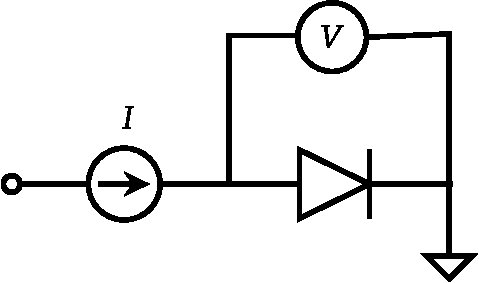
\includegraphics[height=2cm,width=3.5cm]{Net-19-30}
\end{figure}
If $V$ is measured using an ideal voltmeter to estimate $T$, the variation of the voltage $V$ as a function of $T$ is best approximated by (in the following $a$ and $b$ are constants)
 \begin{tasks}(4)
	\task[\textbf{a.}] $a T^{2}+b$
	\task[\textbf{b.}] $a T+b$
	\task[\textbf{c.}] $a T^{3}+b$
	\task[\textbf{d.}] $a T+b T^{2}$
\end{tasks}
\begin{answer}
	\begin{align*}
	I&=k T^{\alpha} e^{-E_{g} / k_{B} T}\left(1+\frac{e V}{k_{B} T}-1\right)\\
	\Rightarrow \frac{e V}{k_{B} T}&=I \frac{T^{-\alpha} e^{E_{g} / k_{B} T}}{k} \Rightarrow \frac{e V}{k_{B} T}=I \frac{T^{-\alpha}}{k}\left(1+\frac{E_{g}}{k_{B} T}\right) \\
	\Rightarrow V&=a T^{-\alpha+1}+b T^{-\alpha} \text {, where } \alpha=0 \Rightarrow V=a T+b
	\end{align*}
		So the correct answer is \textbf{Option (b)}
\end{answer}
\item A circuit constructed using op-amp, resistor $R_{1}=1 k \Omega$ and capacitors $C_{1}=1 \mu F$ and $C_{2}=0.1 \mu F$ is shown in the figure below.
\begin{figure}[H]
	\centering
	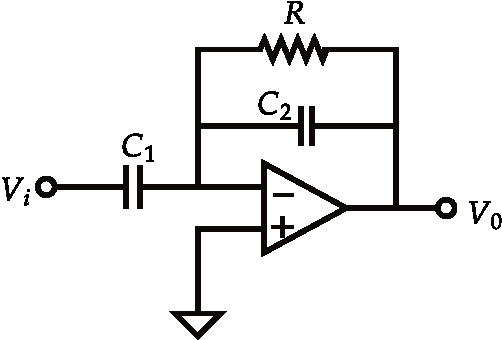
\includegraphics[height=3cm,width=4.5cm]{Net-19-31}
\end{figure}
This circuit will act as a
 \begin{tasks}(2)
	\task[\textbf{a.}]High pass filter
	\task[\textbf{b.}]Low pass filter
	\task[\textbf{c.}]Band pass filter
	\task[\textbf{d.}]Band reject filter 
\end{tasks}
\begin{answer}
	\begin{align*}
	\frac{v_{0}}{v_{i}}&=-\frac{Z_{F}}{Z_{1}}=-\frac{\frac{R_{1} X_{C_{2}}}{R_{1}+X_{C_{2}}}}{X_{C_{1}}}=-\frac{R_{1}}{R_{1} / X_{C_{2}}+1} \times \frac{1}{1 / J \omega C_{1}}\\
	\Rightarrow \frac{v_{0}}{v_{i}}&=-\frac{R_{1} j \omega C_{1}}{R_{1} \times j \omega C_{2}+1}=\frac{R_{1} \omega C_{1}}{\sqrt{1+R_{1}^{2} \omega^{2} C_{2}^{2}}} \frac{e^{-j \theta_{1}}}{e^{j \theta_{2}}} \\
	\Rightarrow\left|\frac{v_{0}}{v_{i}}\right|&=\frac{R_{1} \omega C_{1}}{\sqrt{1+R_{1}^{2} \omega^{2} C_{2}^{2}}}=\frac{R_{1} C_{1}}{\sqrt{1 / \omega^{2}+R_{1}^{2} C_{2}^{2}}}\\
\text{	If }\omega &\rightarrow 0,\left|\frac{v_{0}}{v_{i}}\right| \rightarrow 0
\text{	and If }\omega \rightarrow \infty,\left|\frac{v_{0}}{v_{i}}\right| \rightarrow \frac{C_{1}}{C_{2}}
	\end{align*}
		So the correct answer is \textbf{Option (a)}
\end{answer}
\item The third-nearest neighbour distance in a BCC (Body Centered Cubic) crystal with lattice constant $a_{0}$ is
 \begin{tasks}(4)
	\task[\textbf{a.}] $a_{0}$
	\task[\textbf{b.}]$\frac{3 a_{0}}{2}$
	\task[\textbf{c.}] $\sqrt{3} a_{0}$
	\task[\textbf{d.}]  $\sqrt{2} a_{0}$
\end{tasks}
\begin{answer}$\left. \right. $\\
	\begin{figure}[H]
		\centering
		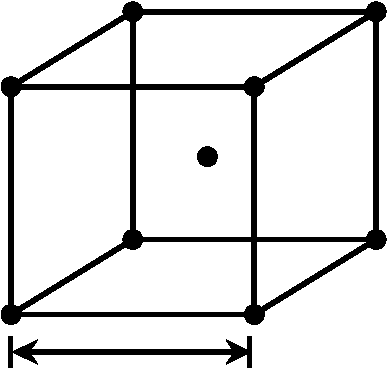
\includegraphics[height=2.5cm,width=2.5cm]{Net-19-37}
	\end{figure}
	\begin{align*}
	\text { The } 1^{\text {st }} \text { nearest atom (I) is at distance }&=\frac{\sqrt{3} a_{0}}{2}=0.87 a_{0}\\
	\text { The } 2^{\text {nd }} \text { nearest atom (II) is at distance }&=a_{0}\\
	\text { The } 3^{\text {rd }} \text { nearest atom (III) is at distance }&=\sqrt{2} a_{0}=1.414 a_{0}
	\end{align*}
		So the correct answer is \textbf{Option (d)}
\end{answer}
\item A bound electron and hole pair interacting via Coulomb interaction in a semiconductor is called an exciton. The effective masses of an electron and a hole are about $0.1 m_{e}$ and $0.5 m_{e}$ respectively, where $m_{e}$ is the rest mass of the electron. The dielectric constant of the semiconductor is 10 . Assuming that the energy levels of the excitons are hydrogenlike, the binding energy of an exciton (in units of the Rydberg constant) is closest to
 \begin{tasks}(4)
	\task[\textbf{a.}]$2 \times 10^{-3}$
	\task[\textbf{b.}]$2 \times 10^{-4}$
	\task[\textbf{c.}]$8 \times 10^{-4}$
	\task[\textbf{d.}]$3 \times 10^{-3}$ 
\end{tasks}
\begin{answer}
	\begin{align*}
	\text { Binding energy of exciton is } E&=(13.6 \mathrm{eV}) \frac{\mu}{m_{e}} \frac{1}{\varepsilon^{2}}\\
\text{were }
	\mu&=\frac{m_{e} \times m_{n}}{m_{e}+m_{n}}=\frac{0.1 m_{e} \times 0.5 m_{e}}{0.1 m_{e}+0.5 m_{e}} \Rightarrow \frac{\mu}{m_{e}}=0.0833\\
	\therefore E&=13.6 \mathrm{eV} \times \frac{0.0833}{100}=13.6 \times 8066 \mathrm{~cm}^{-1} \times 8.33 \times 10^{-4}=9.14 \mathrm{~cm}\\
	\frac{E}{R_{H}}&=\frac{91.4 \mathrm{~cm}^{-1}}{1.097 \times 10^{5} \mathrm{~cm}^{-1}}=8.33 \times 10^{-4}
	\end{align*}
		So the correct answer is \textbf{Option (c)}
\end{answer}
\item Consider an array of atoms in one dimension with an ensemble averaged periodic density distribution as shown in the figure.
\begin{figure}[H]
	\centering
	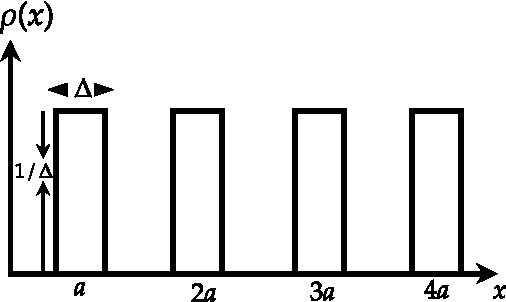
\includegraphics[height=3cm,width=5cm]{Net-19-32}
\end{figure}
If $k$ is the wave number and $S(k, \Delta)$ denotes the Fourier transform of the densitydensity correlation function, the ratio $\frac{S(k, \Delta)}{S(k, 0)}$ is
 \begin{tasks}(4)
	\task[\textbf{a.}] $\cos \left(\frac{k \Delta}{2}\right)$
	\task[\textbf{b.}] $\cos ^{2}\left(\frac{k \Delta}{2}\right)$
	\task[\textbf{c.}] $\frac{2}{k \Delta} \sin \left(\frac{k \Delta}{2}\right)$
	\task[\textbf{d.}] $\frac{4}{k^{2} \Delta^{2}} \sin ^{2}\left(\frac{k \Delta}{2}\right)$
\end{tasks}
\begin{answer}
	\begin{align*}
	\rho(x) \Leftrightarrow s(k, \Delta) \quad& \text { Fourier Transform Pairs }\\
	S(k, \Delta)&=\sum_{n=1}^{\infty} \int_{n a-\frac{\Delta}{2}}^{n a+\frac{\Delta}{2}} \frac{1}{\Delta} e^{i k x} d x \\
	&=\left.\sum_{n=1}^{\infty} \frac{1}{\Delta i k} e^{i k x}\right|_{n a-\frac{\Delta}{2}} ^{n a+\frac{\Delta}{2}}\\
	s(k, \Delta)&=\sum_{n=1}^{\infty} \frac{1}{\Delta i k}\left[e^{i k\left(n a+\frac{\Delta}{2}\right)}-e^{i k\left(n a-\frac{\Delta}{2}\right)}\right] \\
	S&=(k, \Delta)=\sum_{n=1}^{\infty} \frac{e^{i k n a}}{\Delta i k} \frac{\left[e^{i k \Delta / 2}-e^{-i k \Delta / 2}\right]}{2 i} 2 i \\
	&=\frac{\sin k \Delta / 2}{\Delta i k} \cdot 2 i \sum_{k=1}^{\infty} e^{i k n a}=\frac{\sin k \Delta / 2}{k \Delta / 2} \cdot \frac{k \Delta / 2 \cdot 2 i}{\Delta i k}\left[e^{i k a}+e^{i 2 k a}+\cdots\right]\\
	s_{\infty}&=\frac{e^{i k a}}{1-e^{i k a}} \\
	S(k, \Delta)&=\frac{\sin k \Delta / 2}{k \Delta / 2} S_{\infty} \quad S(k, 0)=S_{\infty} \\
	\frac{S(k, \Delta)}{S(k, 0)}&=\frac{2 \sin k \Delta / 2}{k \Delta}
	\end{align*}
	So the correct answer is \textbf{Option (c)}
\end{answer}
\item A doubly charged ion in the angular momentum state $\left(J=2, J_{3}=1\right)$ meets a gas of polarized electrons $\left(S_{3}=\frac{1}{2}\right)$ and gets neutralized. If the orbital angular momentum transferred in the process is zero, the probability that the neutral atom is in the $\left(J=2, J_{3}=2\right)$ state is
 \begin{tasks}(4)
	\task[\textbf{a.}] $\frac{2}{5}$
	\task[\textbf{b.}]$\frac{2}{3}$
	\task[\textbf{c.}]$\frac{1}{5}$
	\task[\textbf{d.}] $\frac{1}{3}$
\end{tasks}
\begin{answer}
	So the correct answer is \textbf{Option (d)}
\end{answer}
\item The range of the inter-atomic potential in gaseous hydrogen is approximately $5 \AA \AA^{\circ}$ In thermal equilibrium, the maximum temperature for which the atom-atom scattering is dominantly $s$-wave, is
 \begin{tasks}(4)
	\task[\textbf{a.}]$500 \mathrm{~K}$
	\task[\textbf{b.}]$100 \mathrm{~K}$
	\task[\textbf{c.}] $1 K$
	\task[\textbf{d.}] $1 m K$
\end{tasks}
\begin{answer}
	So the correct answer is \textbf{Option (c)}
\end{answer}
\item The energy levels corresponding to the rotational motion of a molecule are $E_{J}=B J(J+1) \mathrm{cm}^{-1}$ where $J=0,1,2, \ldots$, and $B$ is a constant. Pure rotational Raman transitions follow the selection rule $\Delta J=0, \pm 2$. When the molecule is irradiated, the separation between the closest Stokes and anti-Stokes lines (in $\mathrm{cm}^{-1}$ ) is
 \begin{tasks}(4)
	\task[\textbf{a.}] $6 B$
	\task[\textbf{b.}]$12 B$
	\task[\textbf{c.}]$4 B$
	\task[\textbf{d.}]$8 B$ 
\end{tasks}
\begin{answer}
	\begin{align*}
	&\text { The selection rules for Raman lines are } \Delta I=\pm 2\\
	&\therefore \overline{\Delta v}=E_{J+2}-E_{J}=B(4 J+6)\\
	&\text{Wave number of stoke's and Anti-stoke's lines are}\\
	&\overline{\Delta v}_{s}=\bar{v}_{0}-\overline{\Delta v}=\bar{v}_{0}-B(4 J+6) \\
	&\overline{\Delta v}_{A s}=\bar{v}_{0}+\overline{\Delta v}=\bar{v}_{0}+B(4 J+6)\\
	&\text{Closest separation between strokes and anti-stokes lines is }\\
	&\overline{\Delta v}=\overline{\Delta v}_{A s}-\overline{\Delta v}_{s}=2 B(4 J+6)=12 B
	\end{align*}
		So the correct answer is \textbf{Option (b)}
\end{answer}
\item The cavity of a He-Ne laser emitting at $632.8 \mathrm{~nm}$, consists of two mirrors separated by a distance of $35 \mathrm{~cm}$. If the oscillations in the laser cavity occur at frequencies within the gain bandwidth of $1.3 \mathrm{GHz}$, the number of longitudinal modes allowed in the cavity is
 \begin{tasks}(4)
	\task[\textbf{a.}]1
	\task[\textbf{b.}]2
	\task[\textbf{c.}]3
	\task[\textbf{d.}] 4
\end{tasks}
\begin{answer}$\left. \right. $
	\begin{figure}[H]
		\centering
		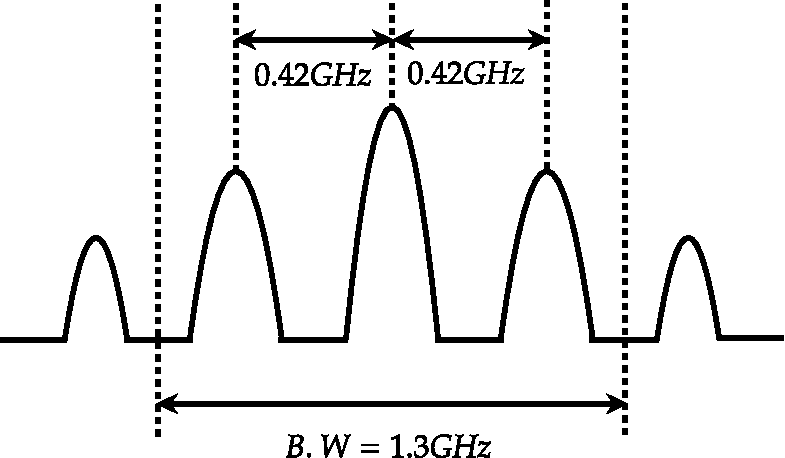
\includegraphics[height=3.5cm,width=6.5cm]{Net-19-38}
	\end{figure}
	\begin{align*}
	\text{The frequency separation }&\text{between two adjacent cavity mode is }\\
\Delta v&=\frac{c}{2 L}=\frac{3 \times 10^{8}}{2 \times 35 \times 10^{-2}}=0.42 \times 10^{9} \mathrm{~Hz}=0.42 \mathrm{GHz}\\
\text { The bandwidth is } \mathrm{B} . \mathrm{W}&=1.3 \mathrm{GHz}
\intertext{Thus, number of longitudinal modes within band width $1.3 \mathrm{GHz}$ are 3 . The correct option is (c)}
	\end{align*}
	So the correct answer is \textbf{Option (c)}
\end{answer}
\item An excited state of a ${ }_{4}^{8}$ Be nucleus decays into two $\alpha$-particles which are in a spinparity $0^{+}$state. If the mean life-time of this decay is $10^{-22} s$, the spin-parity of the excited state of the nucleus is
 \begin{tasks}(4)
	\task[\textbf{a.}]$2^{+}$
	\task[\textbf{b.}]$3^{+}$
	\task[\textbf{c.}]$0^{-}$
	\task[\textbf{d.}]$4^{-}$ 
\end{tasks}
\begin{answer}
 The parity angular momentum selection rule in $\alpha$-decay says that, if the initial and final particles are same, the $I_{\alpha}$ must be even; if the parties are different, then $I_{\alpha}$ must be odd.\\
The ground state is $0^{+}$thus spin-parity of excited state must be $2^{+}$.\\
So the correct answer is \textbf{Option (a)}
\end{answer}
\item The elastic scattering of a neutrino $v_{e}$ by an electron $e^{-}$, i.e. the reaction $v_{e}+e^{-} \rightarrow v_{e}+e^{-}$can be described by the interaction Hamiltonian
$$
H_{\text {int }}=\frac{1}{\sqrt{2}} G_{F} \int d^{3} x\left(\bar{\psi}_{e}(x) \gamma^{\mu} \psi_{v e}(x)\right)\left(\bar{\psi}_{v e}(x) \gamma_{\mu} \psi_{e}(x)\right)
$$
The cross-section of the above process depends on the centre of mass energy $E$, as
 \begin{tasks}(4)
	\task[\textbf{a.}]$\frac{1}{E^{2}}$
	\task[\textbf{b.}]$E^{2}$
	\task[\textbf{c.}]$E$
	\task[\textbf{d.}]$\sqrt{E}$ 
\end{tasks}
\begin{answer}
	So the correct answer is \textbf{Option (b)}
\end{answer}
\item  The mean life-time of the following decays:\\
$\rho_{0} \rightarrow \pi^{+}+\pi^{-}, \pi^{0} \rightarrow \gamma+\gamma, \mu^{-} \rightarrow e^{-}+\bar{v}_{e}+v_{\mu}$, are $\tau_{\rho}, \tau_{\pi}$ and $\tau_{\mu}$ respectively.
They satisfy
 \begin{tasks}(2)
	\task[\textbf{a.}]$\tau_{\pi}<\tau_{\rho}<\tau_{\mu}$
	\task[\textbf{b.}]$\tau_{\mu}<\tau_{\rho}<\tau_{\pi}$
	\task[\textbf{c.}]$\tau_{\rho}<\tau_{\pi}<\tau_{\mu}$
	\task[\textbf{d.}]$\tau_{\rho}<\tau_{\mu}<\tau_{\pi}$ 
\end{tasks}
\begin{answer}
	 The characteristic time for strong, electromagnetic and weak interaction are 
	\begin{align*}
	&\approx 10^{-23} \mathrm{sec}, 10^{-21} \mathrm{sec}\text{ and } 10^{-11} \mathrm{sec}\\
	&\rho_{0} \rightarrow \pi^{+}+\pi^{-}\text{is strong interaction with }\tau_{\rho} \simeq 10^{-23} \mathrm{sec}\\
	&\pi^{0} \rightarrow \gamma+\gamma\text{ is electromagnetic interaction with }\tau_{\pi} \simeq 10^{-21} \mathrm{sec}\\
	&\mu^{-} \rightarrow e^{-}+\bar{v}_{e}+v_{\mu}\text{ is weak interaction with }\tau_{\mu} \simeq 10^{-11} \mathrm{sec}\\
	&\text{Thus, }\tau_{\rho}<\tau_{\pi}<\tau_{\mu}.\text{ The correct option is (c)}
	\end{align*}
	So the correct answer is \textbf{Option (c)}
\end{answer}
\end{enumerate}